%===============================================================================
% LaTeX sjabloon voor de bachelorproef toegepaste informatica aan HOGENT
% Meer info op https://github.com/HoGentTIN/latex-hogent-report
%===============================================================================

\documentclass[dutch,dit,thesis]{hogentreport}

%% Pictures to include in the text can be put in the graphics/ folder
\graphicspath{{graphics/}}

%% For source code highlighting, requires pygments to be installed
%% Compile with the -shell-escape flag!
\usepackage[section]{minted}
\usemintedstyle{solarized-light}
\definecolor{bg}{RGB}{253,246,227} %% Set the background color of the codeframe

%% Change this line to edit the line numbering style:
\renewcommand{\theFancyVerbLine}{\ttfamily\scriptsize\arabic{FancyVerbLine}}

%% Macro definition to load external java source files with \javacode{filename}:
\newmintedfile[javacode]{java}{
    bgcolor=bg,
    fontfamily=tt,
    linenos=true,
    numberblanklines=true,
    numbersep=5pt,
    gobble=0,
    framesep=2mm,
    funcnamehighlighting=true,
    tabsize=4,
    obeytabs=false,
    breaklines=true,
    mathescape=false
    samepage=false,
    showspaces=false,
    showtabs =false,
    texcl=false,
}

% Other packages not already included can be imported here
\usepackage{xcolor} % Voeg het xcolor-pakket toe voor kleurdefinities
\usepackage{pdfpages}

% Definieer kleuren voor syntax highlighting
\definecolor{codebg}{RGB}{240, 240, 240} % Achtergrondkleur van de code
\definecolor{codecomment}{RGB}{106, 153, 85} % Kleur van opmerkingen
\definecolor{codekeyword}{RGB}{166, 35, 35} % Kleur van keywords
\definecolor{codestring}{RGB}{42, 0, 255} % Kleur van strings

% Configureer minted
\usemintedstyle{default} % Kies een stijl voor de code (bijv. 'default', 'vs', 'friendly', 'colorful', etc.)
\setminted{
    bgcolor=codebg, % Achtergrondkleur
    fontsize=\footnotesize, % Lettergrootte
    linenos=true, % Plaatsing van regelnummers
    breaklines=true, % Automatisch afbreken van lange regels
    frame=leftline, % Plaatsing van frame rondom de code (leftline = lijn aan de linkerkant)
    framesep=10pt, % Afstand tussen frame en code
    rulecolor=\color{black}, % Kleur van het frame
    numbersep=15pt, % Afstand tussen regelnummers en code (aangepast)
    xleftmargin=0pt, % Marge aan de linkerkant van het kader (op 0pt zetten)
}


%%---------- Document metadata -------------------------------------------------
\author{Truye Bjorn}
\supervisor{Mevr. S. Lambert}
\cosupervisor{Dhr. D. Matthijs}
\title
    {Strategieën om de overname van bestaande webshops naar WordPress met WooCommerce te stroomlijnen: een onderzoek en proof-of-concept.}
\academicyear{\advance\year by -1 \the\year--\advance\year by 1 \the\year}
\examperiod{1}
\degreesought{\IfLanguageName{dutch}{Professionele bachelor in de toegepaste informatica}{Bachelor of applied computer science}}
\partialthesis{false} %% To display 'in partial fulfilment'
%\institution{Internshipcompany BVBA.}

%% Add global exceptions to the hyphenation here
\hyphenation{back-slash}

%% The bibliography (style and settings are  found in hogentthesis.cls)
\addbibresource{bachproef.bib}            %% Bibliography file
\addbibresource{../voorstel_v2/TruyeBjorn-BPvoorstel.bib} %% Bibliography research proposal
\defbibheading{bibempty}{}

%% Prevent empty pages for right-handed chapter starts in twoside mode
\renewcommand{\cleardoublepage}{\clearpage}

\renewcommand{\arraystretch}{1.2}

%% Content starts here.
\begin{document}

%---------- Front matter -------------------------------------------------------

\frontmatter

\hypersetup{pageanchor=false} %% Disable page numbering references
%% Render a Dutch outer title page if the main language is English
\IfLanguageName{english}{%
    %% If necessary, information can be changed here
    \degreesought{Professionele Bachelor toegepaste informatica}%
    \begin{otherlanguage}{dutch}%
       \maketitle%
    \end{otherlanguage}%
}{}

%% Generates title page content
\maketitle
\hypersetup{pageanchor=true}

%%=============================================================================
%% Voorwoord
%%=============================================================================

\chapter*{\IfLanguageName{dutch}{Woord vooraf}{Preface}}%
\label{ch:voorwoord}

%% TODO:
%% Het voorwoord is het enige deel van de bachelorproef waar je vanuit je
%% eigen standpunt (``ik-vorm'') mag schrijven. Je kan hier bv. motiveren
%% waarom jij het onderwerp wil bespreken.
%% Vergeet ook niet te bedanken wie je geholpen/gesteund/... heeft
Graag wil ik van deze gelegenheid gebruikmaken om mijn promotor S. Lambert te bedanken voor de talloze feedback momenten, en om mijn co-promotor D. Matthijs te bedanken voor het aanbieden van deze interessante bedrijfscasus. Als webontwikkelaar die al enkele webshops gemaakt heeft, sprak deze uitdaging mij direct aan.
\\\\
Afgelopen periode van technologische vooruitgang was, voornamelijk op AI-vlak, een heel erg leerzaam en boeiende ervaring. Desondanks de vele literatuurstudies die ongetwijfeld heel snel zullen achterhaald worden, bleef het fascinerend om te zien hoe alles enorm snel aan het evolueren is. Het is waar dat we op technologisch vlak snel veranderingen meemaken, maar een AI-evolutie zoals deze zagen we allemaal niet aankomen. Ondertussen heeft bijna heel de wereld over ChatGPT gehoord, of al eens gebruikt. Nooit had ik mij kunnen voorstellen dat gedurende heel mijn stageperiode een persoonlijke assistent mij kon assisteren bij het programmeren. Afgelopen maanden was er elke dag iets nieuws over AI te vertellen en het brengt tot op vandaag nog altijd veel media-aandacht met zich mee. Bedrijven zijn volop aan de gang met bestaande tools van AI te voorzien om ons leven eenvoudiger te maken. Binnenkort hoeven we zelfs onze eigen e-mails niet meer te schrijven.
\\\\
Als iemand geboren in de jaren '90 en met een grote passie voor technologie is dit echt adembenemend om mee te mogen maken. Het is aan de ene kant alarmerend maar tegelijkertijd ook fascinerend hoeveel werk voor ons op zoveel vlakken geautomatiseerd kan worden. Bij aanvang van deze paper was het niet de bedoeling om met AI te werken, maar het is heel erg duidelijk geworden dat AI hierbij het meeste kan helpen.
\\\\
Op moment van schrijven is het nog niet helemaal duidelijk hoever we staan in deze evolutie maar één ding is zeker: AI is de toekomst.
%%=============================================================================
%% Samenvatting
%%=============================================================================

% TODO: De "abstract" of samenvatting is een kernachtige (~ 1 blz. voor een
% thesis) synthese van het document.
%
% Een goede abstract biedt een kernachtig antwoord op volgende vragen:
%
% 1. Waarover gaat de bachelorproef?
% 2. Waarom heb je er over geschreven?
% 3. Hoe heb je het onderzoek uitgevoerd?
% 4. Wat waren de resultaten? Wat blijkt uit je onderzoek?
% 5. Wat betekenen je resultaten? Wat is de relevantie voor het werkveld?
%
% Daarom bestaat een abstract uit volgende componenten:
%
% - inleiding + kaderen thema
% - probleemstelling
% - (centrale) onderzoeksvraag
% - onderzoeksdoelstelling
% - methodologie
% - resultaten (beperk tot de belangrijkste, relevant voor de onderzoeksvraag)
% - conclusies, aanbevelingen, beperkingen
%
% LET OP! Een samenvatting is GEEN voorwoord!

%%---------- Nederlandse samenvatting -----------------------------------------

\IfLanguageName{english}{%
\selectlanguage{dutch}
\chapter*{Samenvatting}
\selectlanguage{english}
}{}

%%---------- Samenvatting -----------------------------------------------------
% De samenvatting in de hoofdtaal van het document

\chapter*{\IfLanguageName{dutch}{Samenvatting}{Abstract}}

De co-promotor D.Matthijs heeft een bedrijf Team Made dat niet alleen websites en webshops bouwt, maar ook overneemt. Het proces van een webshop over te nemen, en om te zetten naar een WordPress met WooCommerce, kan veel tijd in beslag nemen. Deze paper doet een onderzoek en houdt een proof-of-concept om dit proces te doen stroomlijnen.
\\\\
Een webshop overnemen is niet zomaar evident en vereist enige programmeerkennis. Er kunnen veel (externe) factoren zorgen voor een complexe overdracht. Klanten moeten hun eigen webshop zelf kunnen beheren, een webshop kan een zeer complexe lay-out hebben, er kunnen reeds veel artikelen aanwezig zijn enzovoort. Hoe kunnen we een overname zo eenvoudig en minst tijdrovend mogelijk maken?
\\\\
Eerst en vooral gaan we kijken naar de huidige middelen op de markt die ons kunnen helpen bij deze problematiek. Vervolgens proberen we met een combinatie van bestaande en eventueel zelf ontwikkelde tools tot een resultaat te komen dat de co-promotor tijd doet winnen. En dat allemaal zonder onder te doen aan kwaliteit. 
\\\\
Het resultaat van deze paper is een volledig geautomatiseerd proces voor de hele opzet en installatie, met zo weinig mogelijk manueel werk voor de co-promotor. Het voorzien van de lay-out en het opvullen van de data, kan met behulp van een groeiend aantal AI-tools veel sneller worden verwezenlijkt.
\\\\
Het is sterk aanbevolen om zoveel mogelijk te laten automatiseren met de tools die WordPress ons aanbiedt. Het overnemen van een webshop blijft echter een proces dat enig manueel werk vergt. Er zal altijd een expert nodig zijn voor het beste resultaat te bekomen. De huidig lopende AI-evolutie biedt op moment van schrijven ons talloze opties aan die alleen maar met de dag beter worden, maar ze zijn niet de eindoplossing.


%KOMEN LATER UITGEBREIDER AAN BOD
%
%Inleiding + kaderen thema:
%\begin{itemize}
%    \item Zeggen wat een CMS is, en wat bijgevolg WordPress is
%    \item Zeggen wat een webshop is, en uitleggen wat WooCommerce is
%    \item Zeggen dat er nog andere opties op de markt bestaan (zowel cms als webshop plugins)
%    \item Uitleg over wat een webshop overname precies is
%\end{itemize}
%
%Probleemstelling
%\begin{itemize}
%    \item Veel opties op de markt (zowel CMS als plugins)
%    \item Momenteel veel manueel werk (voor co-promotor) bij een webshop overname
%    \item Doelgroep = mijn co-promotor zijn bedrijf, maar ook andere IT-bedrijven die webshops overnemen?
%    \item Veiligheid bespreken
%    \item Schendig van rechten bij overname bespreken (GDPR)
%    \item Future-proof tool (bv. code dat breekt bij updates)
%\end{itemize}
%
%(centrale) onderzoeksvraag
%\begin{itemize}
%    \item --> hoe kan dit proces eenvoudiger?
%    \item Vooral nu erg belangrijk om te zien of AI (deels) een oplossing kan bieden
%\end{itemize}
%
%onderzoeksdoelstelling:
%\begin{itemize}
%    \item Kijken welke stappen eenvoudiger / geautomatiseerd kunnen
%    \item Co-promotor wilt WP en WC gebruiken, wel ok? Geen betere alternatieven? Kort analyseren waarom
%    \item Bestaat er reeds een (AI) tool die dit (deels) kan?
%    \item Indien ja, kan mijn co-promotor dit gebruiken? Zijn er limieten?
%    \item Indien neen, kan een tool geschreven worden die dit (deels) kan?
%    \item Beoogde resultaat: een (zelfgeschreven) tool die het gemakkelijker maakt / tijd bespaart om webshops over te nemen
%    \item Criteria voor succes: overname gaat sneller, bespaart kosten (bv. met goedkopere plugins)
%\end{itemize}
%
%methodologie:
%\begin{itemize}
%    \item Bestaande (AI) tools overlopen + testen op hun limieten
%    \item Kijken of een tool alles kan, of een combo van meerdere nodig is
%\end{itemize}
%
%resultaten (beperk tot de belangrijkste, relevant voor de onderzoeksvraag):
%\begin{itemize}
%    \item kan ik pas na de literatuurstudie neerschrijven?
%    \item komen hier mijn verwachtingen te staan?
%\end{itemize}
%
%conclusies, aanbevelingen, beperkingen
%\begin{itemize}
%    \item kan ik pas op het einde schrijven?
%\end{itemize}

%---------- Inhoud, lijst figuren, ... -----------------------------------------

\tableofcontents

% In a list of figures, the complete caption will be included. To prevent this,
% ALWAYS add a short description in the caption!
%
%  \caption[short description]{elaborate description}
%
% If you do, only the short description will be used in the list of figures

\listoffigures

% If you included tables and/or source code listings, uncomment the appropriate
% lines.
%\listoftables
%\listoflistings

% Als je een lijst van afkortingen of termen wil toevoegen, dan hoort die
% hier thuis. Gebruik bijvoorbeeld de ``glossaries'' package.
% https://www.overleaf.com/learn/latex/Glossaries

%---------- Kern ---------------------------------------------------------------

\mainmatter{}

% De eerste hoofdstukken van een bachelorproef zijn meestal een inleiding op
% het onderwerp, literatuurstudie en verantwoording methodologie.
% Aarzel niet om een meer beschrijvende titel aan deze hoofdstukken te geven of
% om bijvoorbeeld de inleiding en/of stand van zaken over meerdere hoofdstukken
% te verspreiden!

%%=============================================================================
%% Inleiding
%%=============================================================================

\chapter{\IfLanguageName{dutch}{Inleiding}{Introduction}}%
\label{ch:inleiding}

%De inleiding moet de lezer net genoeg informatie verschaffen om het onderwerp te begrijpen en in te zien waarom de onderzoeksvraag de moeite waard is om te onderzoeken. In de inleiding ga je literatuurverwijzingen beperken, zodat de tekst vlot leesbaar blijft. Je kan de inleiding verder onderverdelen in secties als dit de tekst verduidelijkt. Zaken die aan bod kunnen komen in de inleiding~\autocite{Pollefliet2011}:
%
%\begin{itemize}
%  \item context, achtergrond
%  \item afbakenen van het onderwerp
%  \item verantwoording van het onderwerp, methodologie
%  \item probleemstelling
%  \item onderzoeksdoelstelling
%  \item onderzoeksvraag
%  \item \ldots
%\end{itemize}

Een webshop is een website waarop goederen en/of diensten worden verkocht. Om een webshop van inhoud te voorzien moet deze zo eenvoudig mogelijk opgevuld worden. Hiervoor bestaan er verschillende tools, waaronder een CMS of contentmanagementsysteem. Hiermee kan met behulp van een inlogsysteem de klant de webshop bewerken, zonder enige programmeerkennis. De co-promotor gebruikt hiervoor WordPress. Standaard is WordPress maar een website voor blogberichten. Via uitbreidingen op deze tool, bekend onder de naam plugins, kan er zo een webshop worden gemaakt. Een bekende plugin die de co-promotor hiervoor gebruikt is WooCommerce. Merk op dat er nog veel andere CMS'en en WordPress plugins bestaan, maar deze niet tot in detail worden besproken in deze paper, aangezien de co-promotor met deze tools zal blijven verder werken. 
\\\\
Het overnemen van een webshop betekent dat je een nieuwe webshop maakt, en zoveel mogelijk van de originele webshop tracht over te nemen. Idealiter worden problemen of mankementen bij deze overname niet meegenomen. Voor de co-promotor betekent dit een nieuwe WordPress met WooCommerce opzetten, en zoveel mogelijk trachten over te nemen van de originele webshop.

\section{\IfLanguageName{dutch}{Probleemstelling}{Problem Statement}}%
\label{sec:probleemstelling}

%Uit je probleemstelling moet duidelijk zijn dat je onderzoek een meerwaarde heeft voor een concrete doelgroep. De doelgroep moet goed gedefinieerd en afgelijnd zijn. Doelgroepen als ``bedrijven,'' ``KMO's'', systeembeheerders, enz.~zijn nog te vaag. Als je een lijstje kan maken van de personen/organisaties die een meerwaarde zullen vinden in deze bachelorproef (dit is eigenlijk je steekproefkader), dan is dat een indicatie dat de doelgroep goed gedefinieerd is. Dit kan een enkel bedrijf zijn of zelfs één persoon (je co-promotor/opdrachtgever).

Team Made, en ook andere bedrijven die aan webshops overnames doen, verliest veel tijd aan zo een overname. Het is ook niet altijd even voor de hand liggend hoeveel tijd en budgettering zo een overname precies in beslag zal nemen. Daarnaast moet de webshop ook op een veilige manier worden opgebouwd, die liefst zo lang mogelijk mee gaat in deze zeer snel groeiende technologische wereld. We willen niet dat een splik splinternieuwe webshop na een paar weken al out-of-date is. We moeten ervoor zorgen dat de code zo future-proof mogelijk is.

\section{\IfLanguageName{dutch}{Onderzoeksvraag}{Research question}}%
\label{sec:onderzoeksvraag}

%Wees zo concreet mogelijk bij het formuleren van je onderzoeksvraag. Een onderzoeksvraag is trouwens iets waar nog niemand op dit moment een antwoord heeft (voor zover je kan nagaan). Het opzoeken van bestaande informatie (bv. ``welke tools bestaan er voor deze toepassing?'') is dus geen onderzoeksvraag. Je kan de onderzoeksvraag verder specifiëren in deelvragen. Bv.~als je onderzoek gaat over performantiemetingen, dan 

Zijn er vandaag de dag genoeg tools aanwezig die dit overnameproces kunnen stroomlijnen? Is er een manier om dit ook voor meerdere klanten tegelijkertijd sneller te laten verlopen? Kan alles met behulp van één tool worden versneld, of moet een combinatie van tools worden gebruikt? Het zijn allemaal vragen die we ons moeten stellen om het overnameproces te willen stroomlijnen.

\section{\IfLanguageName{dutch}{Onderzoeksdoelstelling}{Research objective}}%
\label{sec:onderzoeksdoelstelling}

%Wat is het beoogde resultaat van je bachelorproef? Wat zijn de criteria voor succes? Beschrijf die zo concreet mogelijk. Gaat het bv.\ om een proof-of-concept, een prototype, een verslag met aanbevelingen, een vergelijkende studie, enz.

Er zal onderzoek worden gedaan naar welke stappen noodzakelijk zijn voor een webshop overname, en hoe deze vereenvoudigd of zelfs geautomatiseerd kunnen worden. Hierbij zullen we kort analyseren of de tools die Team Made gebruikt, namelijk WordPress en WooCommerce, betere alternatieven hebben of niet. We wensen dat Team Made een (combinatie van) (zelfgeschreven) tool(s) kan gebruiken om zijn bestaande workflow te optimaliseren. Als een overname sneller gaat, of goedkopere alternatieven te bieden heeft die niet inboeten op tijd en kwaliteit, dan zitten we op het juiste spoor.

\section{\IfLanguageName{dutch}{Opzet van deze bachelorproef}{Structure of this bachelor thesis}}%
\label{sec:opzet-bachelorproef}

% Het is gebruikelijk aan het einde van de inleiding een overzicht te
% geven van de opbouw van de rest van de tekst. Deze sectie bevat al een aanzet
% die je kan aanvullen/aanpassen in functie van je eigen tekst.

De rest van deze bachelorproef is als volgt opgebouwd:

In Hoofdstuk~\ref{ch:stand-van-zaken} wordt een overzicht gegeven van de stand van zaken binnen het onderzoeksdomein, op basis van een literatuurstudie.

In Hoofdstuk~\ref{ch:methodologie} wordt de methodologie toegelicht en worden de gebruikte onderzoekstechnieken besproken om een antwoord te kunnen formuleren op de onderzoeksvragen.

In Hoofdstuk~\ref{ch:stappenplan} wordt een kort overzicht gegeven van de stappen die men moet ondernemen voor het maken en overnemen van een webshop.

In Hoofdstuk~\ref{ch:conclusie}, tenslotte, wordt de conclusie gegeven en een antwoord geformuleerd op de onderzoeksvragen. Daarbij wordt ook een aanzet gegeven voor toekomstig onderzoek binnen dit domein.

\chapter{\IfLanguageName{dutch}{Stand van zaken}{State of the art}}%
\label{ch:stand-van-zaken}

% Tip: Begin elk hoofdstuk met een paragraaf inleiding die beschrijft hoe
% dit hoofdstuk past binnen het geheel van de bachelorproef. Geef in het
% bijzonder aan wat de link is met het vorige en volgende hoofdstuk.

% Pas na deze inleidende paragraaf komt de eerste sectiehoofding.

%Dit hoofdstuk bevat je literatuurstudie. De inhoud gaat verder op de inleiding, maar zal het onderwerp van de bachelorproef *diepgaand* uitspitten. De bedoeling is dat de lezer na lezing van dit hoofdstuk helemaal op de hoogte is van de huidige stand van zaken (state-of-the-art) in het onderzoeksdomein. Iemand die niet vertrouwd is met het onderwerp, weet nu voldoende om de rest van het verhaal te kunnen volgen, zonder dat die er nog andere informatie moet over opzoeken \autocite{Pollefliet2011}.
%
%Je verwijst bij elke bewering die je doet, vakterm die je introduceert, enz.\ naar je bronnen. In \LaTeX{} kan dat met het commando \texttt{$\backslash${textcite\{\}}} of \texttt{$\backslash${autocite\{\}}}. Als argument van het commando geef je de ``sleutel'' van een ``record'' in een bibliografische databank in het Bib\LaTeX{}-formaat (een tekstbestand). Als je expliciet naar de auteur verwijst in de zin, gebruik je \texttt{$\backslash${}textcite\{\}}.
%Soms wil je de auteur niet expliciet vernoemen, dan gebruik je \texttt{$\backslash${}autocite\{\}}. In de volgende paragraaf een voorbeeld van elk.
%
%\textcite{Knuth1998} schreef een van de standaardwerken over sorteer- en zoekalgoritmen. Experten zijn het erover eens dat cloud computing een interessante opportuniteit vormen, zowel voor gebruikers als voor dienstverleners op vlak van informatietechnologie~\autocite{Creeger2009}.

\section{De onverwachtse groei van AI}
AI is de afkorting van Artificiële Intelligentie en is op moment van schrijven het meest besproken onderwerp wereldwijd op vlak van technologie. Het is heel erg duidelijk dat tijdens het schrijven van deze paper veel bedrijven zich volledig zijn gaan focussen op AI. Zo heeft Google een hele uitgebreide \href{https://ai.google/why-ai/}{webpagina} uitgebracht begin 2023 waarom ze die keuze hebben gemaakt en wat hun toekomstperspectieven in verband met AI zijn.
\\\\
Er zijn sinds het schrijven van deze paper gigantisch veel nieuwe AI-tools voor het eerste publiek toegankelijk gemaakt. Bijgevolg zullen helaas veel aspecten van deze literatuurstudie reeds achterhaald zijn bij de oplevering van deze paper. Wereldwijd zijn mensen door de overvloed van AI-tools zoals ChatGPT, de vernieuwde Bing zoekmachine en AutoGPT beginnen realiseren wat AI allemaal te bieden heeft.
\\\\
Daarnaast is er een constante druk bij de bedrijven om de beste resultaten op te leveren. Een bekend voorbeeld hiervan is Google die een hele grote druk op zich kreeg om hun zoekmachine te verbeteren wanneer Samsung overwoog om hun standaard zoekmachine op mobiele toestellen te veranderen \autocite{Paris2023}. Bijgevolg is er een gigantische AI-strijd ontstaan (en op moment van schrijven nog steeds bezig). 
\\\\
Door deze gigantische stroomversnelling in AI zullen in deze paper een aantal AI-tools kort vermeld worden, maar niet tot in detail worden besproken. AI werkt, zoals kort in deze YouTube-film \autocite{Grey2017} beschreven, door constant zichzelf te testen en te evalueren. Aangezien er wereldwijd miljoenen gebruikers de AI-tools aan het trainen zijn door bv. feedback te geven aan ChatGPT zijn antwoorden, worden deze tools heel erg snel verbeterd. Hierdoor kunnen deze tools op een relatief korte tijd aanzienlijk veel beter worden. Bijgevolg moeten alle verworven AI-resultaten binnen deze paper met een grote korrel zout worden genomen.
\\\\
\section{Eervolle vermeldingen}
Dit zijn AI-tools die sinds de start van deze paper ontstaan zijn, in beta zijn gekomen of gedemonstreerd werden en best nauwkeurig in de gaten worden gehouden door de co-promotor in de nabije toekomst. Hou er rekening mee dat niet elke tool gratis is en prijzen doorheen de loop van tijd kunnen wijzigen.
\\\\
\subsection{Microsoft JARVIS}
Microsoft heeft op \href{https://github.com/microsoft/JARVIS}{GitHub een project genaamd JARVIS} openbaar gezet. Op moment van schrijven is de code nog niet raadpleegbaar. De tool is in staat om afbeeldingen te genereren, te laten variëren op bestaande afbeeldingen en de afbeelding te laten omschrijven. Het belangrijkste is dat objecten op afbeeldingen kunnen herkend worden, iets wat ideaal zou zijn om lay-out elementen te laten overnemen.
\begin{figure}
    \caption{'JARVIS kan afbeeldingen genereren en omschrijven'}
    \begin{center}
        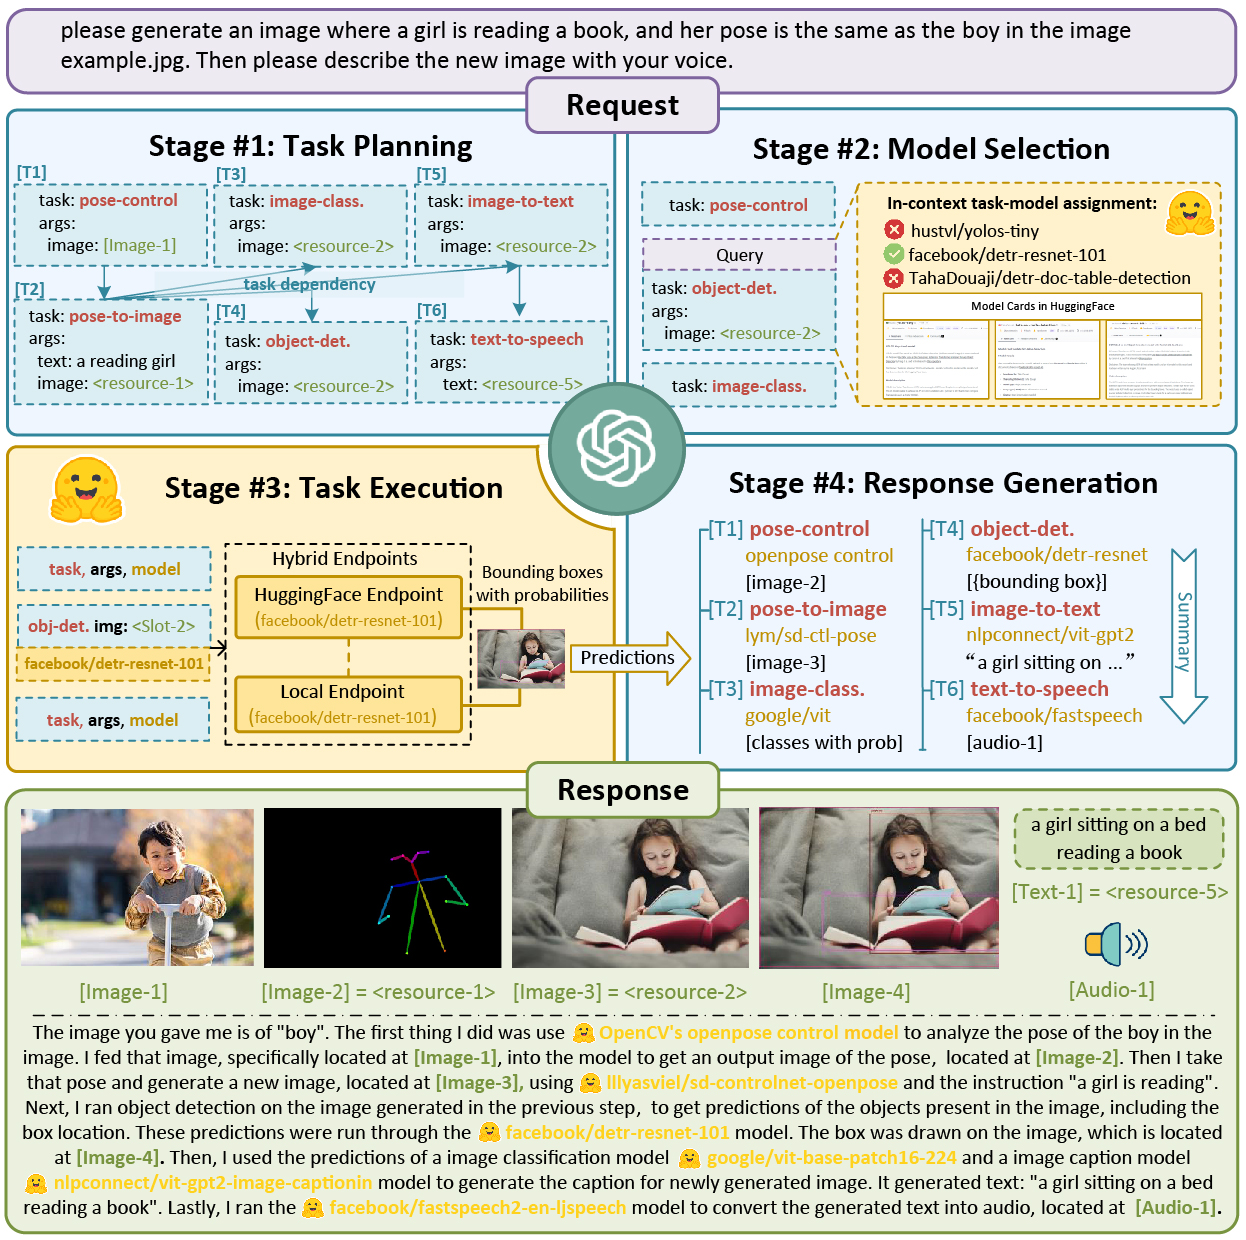
\includegraphics[width=\textwidth, height=\textheight, keepaspectratio]{jarvis_overview}
    \end{center}
\end{figure}
\begin{figure}
    \caption{'JARVIS kan objecten op afbeeldingen herkennen'}
    \begin{center}
        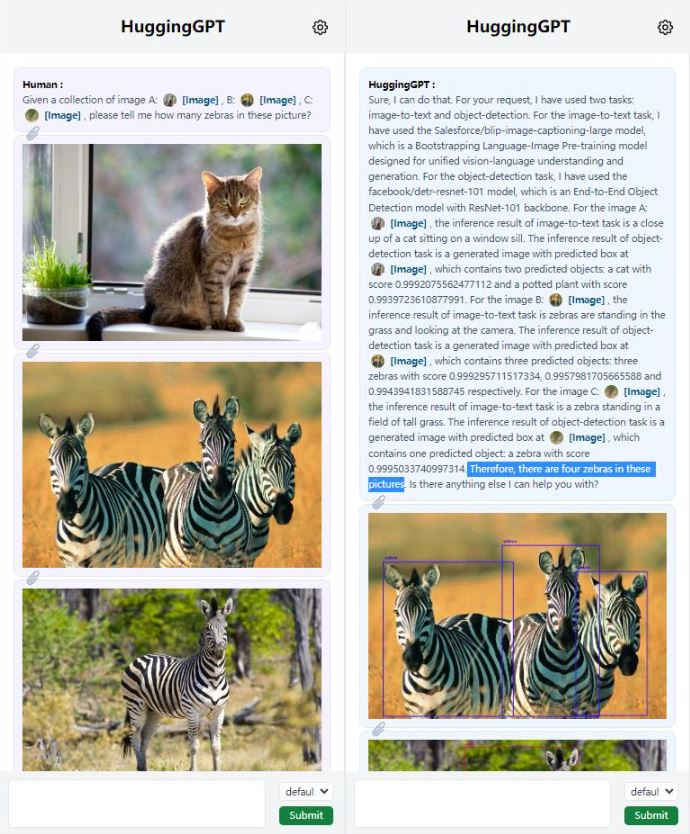
\includegraphics[width=\textwidth, height=\textheight, keepaspectratio]{jarvis_overview_2}
    \end{center}
\end{figure}
\subsection{Elementor AI}
Er zijn talloze manieren om de gebruikerservaring met WordPress voor zowel de programmeurs als eindgebruikers eenvoudiger te maken. Een voorbeeld hiervan is Elementor. Het bedrijf staat o.a. bekend voor WordPress hosting, een builder om websites te maken en hun plugin die websites met een Elementor thema visueel kan aanpassen.
\\\\
Op 3 april 2023 bracht Elementor een tweede Roadmap Event \autocite{Laster2023} uit waar ze hun Elementor AI voorstelden. Het is in staat om tekst te vertalen in code en kan gebruikt worden om elementen aan te passen zonder enige programmeerkennis. Veel meer extra informatie over functionaliteiten en prijzen zijn er op moment van schrijven nog niet over terug te vinden.
\subsection{Auto-GPT}
Het project \href{https://github.com/Significant-Gravitas/Auto-GPT}{Auto-GPT: An Autonomous GPT-4 Experiment} is op GitHub raadpleegbaar en is op moment van schrijven nog een experiment. De laatste demo is momenteel van 16 april 2023 waarin de tool een webpagina analyseert om een samenvatting van de inhoud te maken en op te slaan in een tekstbestand.
\\\\
Een mogelijke toepassing van deze tool is het analyseren van een reeds bestaande webshop en de inhoud ervan in code teruggeven op een manier dat direct in een bestaand thema kan worden geïmplementeerd.
\subsection{AgentGPT} 
Deze tool is op moment van schrijven nog in beta. Het principe van \href{https://agentgpt.reworkd.ai/nl}{AgentGPT} is simplistisch uitgelegd dat je een complexe opdracht stelt aan de tool, die het vervolgens opdeelt in kleinere taken en elke taak toewijst aan een AI-agent. Die AI-agent krijgt enkel en alleen maar de rechten die hij nodig heeft. Zo kan een agent die iets moet opzoeken bv. geen betalingen uitvoeren. 
\\\\
Sinds begin mei 2023 is het mogelijk om ook eigen taken toe te voegen. Bij de oorspronkelijke release van deze tool was dit nog niet het geval, en was Godmode een alternatief hiervoor. Momenteel lukt het niet om websites volledig te clonen zonder een eigen API-sleutel te voorzien, en bijgevolg te betalen. Het commando “Clone the webshop https://www.coureurlocal.be/” geeft het volgende resultaat:
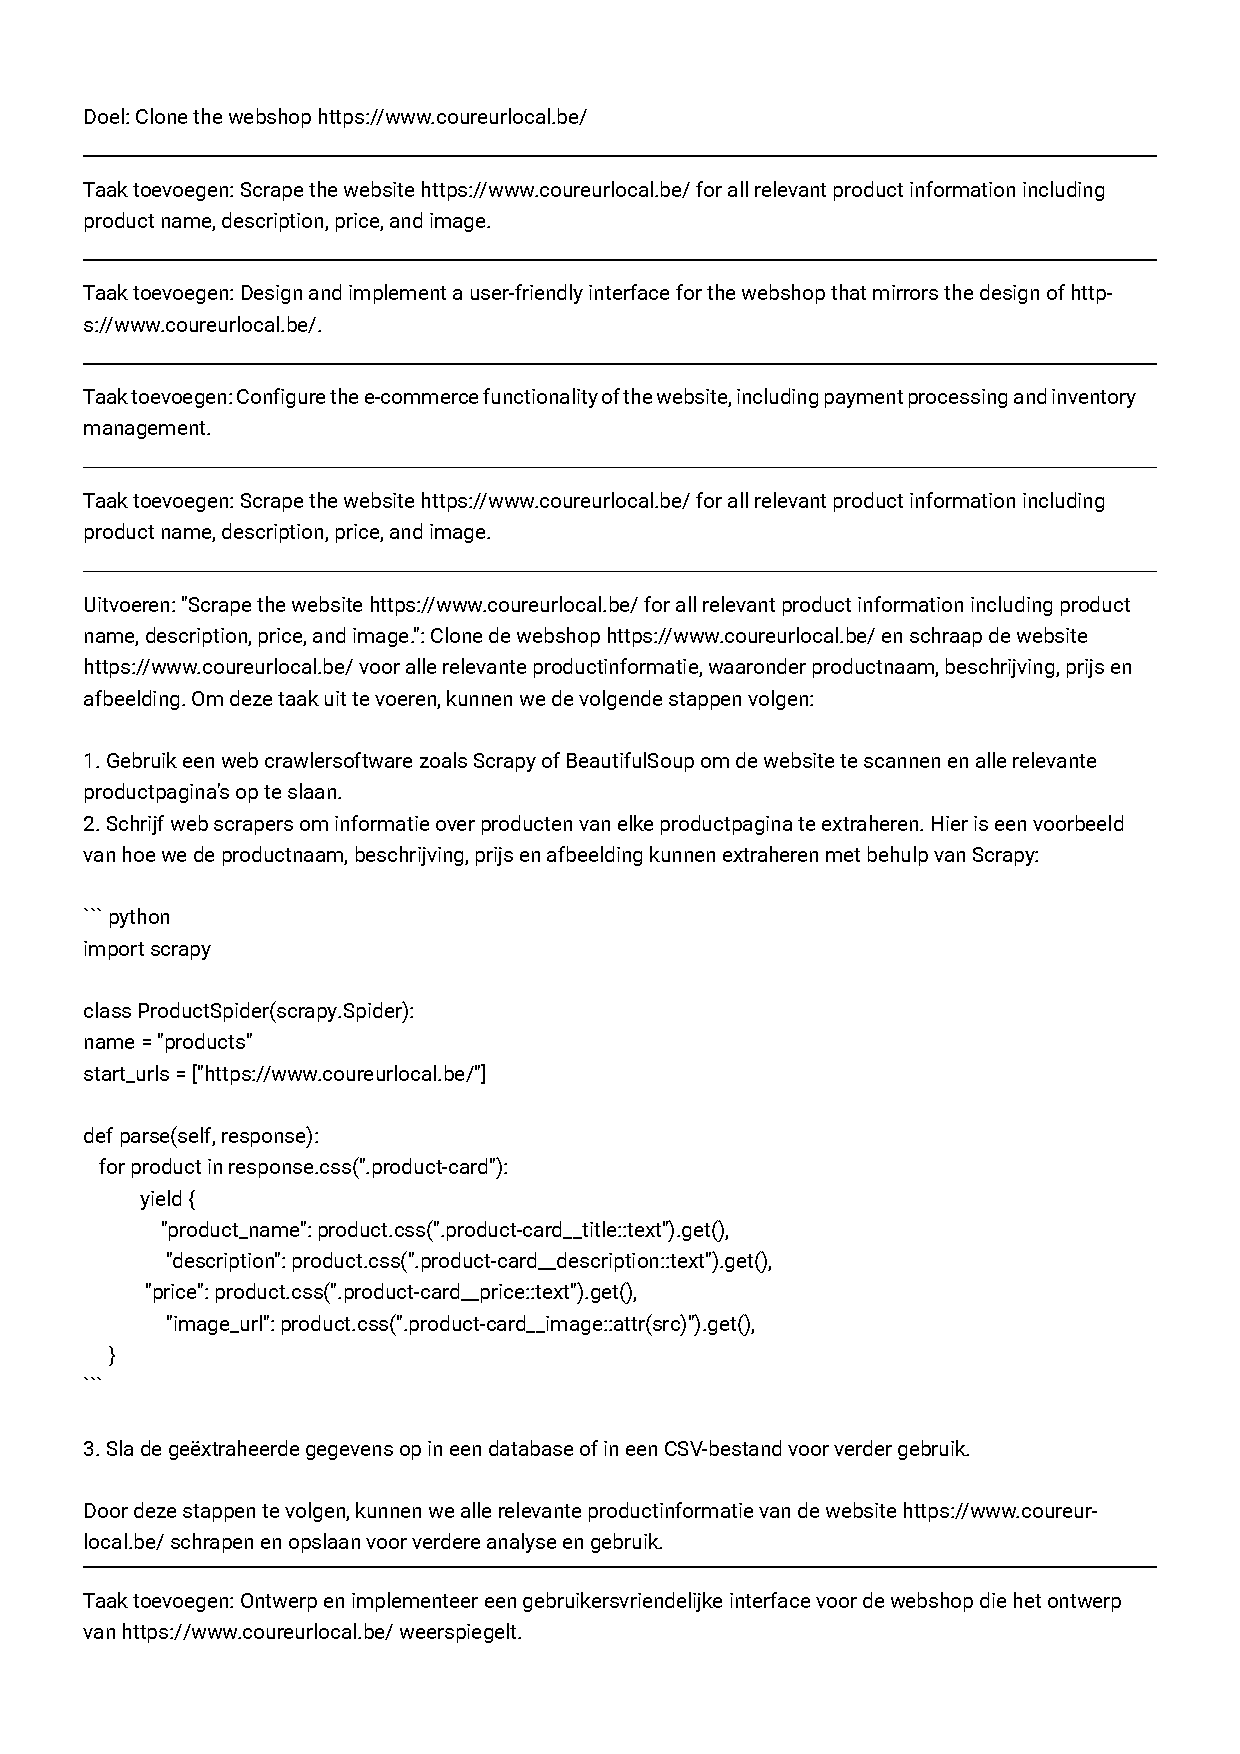
\includepdf[pages=-]{agentGPT_coureur_local.pdf}
\subsection{Godmode}
\href{https://godmode.space}{Godmode} is een alternatief voor AgentGPT dat eerder de mogelijkheid had om zelf taken toe te voegen. De tool laat toe om na elke taak feedback te geven en vereist bijgevolg ook telkens actie van de gebruiker. Uitvoerig gebruik is helaas gratis niet mogelijk en geeft telkens de melding “Due to very high use, please provide your own OpenAI key to continue”. Op moment van schrijven staan \href{https://docs.google.com/forms/d/e/1FAIpQLSdfKYSOEifsbKsfx365zZ0TuZpE9ovLUcAwpGY3NFNRg6l25w/viewform}{inschrijvingen voor Godmode versie 2} open.
\\\\
\subsection{Code Interpreter Plugin}
Dit is een codeer plugin voor ChatGPT waarvan de auteur nog geen toegang heeft verkregen. De plugin biedt ChatGPT een werkende Python-interpreter aan in een sandbox-omgeving. Het zou zelfs in staat zijn om basis video editing te doen en kleine video's te genereren \autocite{Jose2023}.
\section{Webshops}
\subsection{Definitie en belang}
Doorheen de afgelopen jaren zijn webshops en online retail alleen maar in populariteit gestegen \autocite{Roggeveen2020}. Zo was tijdens de coronapandemie, wanneer sociaal contact verboden was, het hebben van een webshop vrij cruciaal. Bedrijven die voornamelijk al een webshop voor Maart 2020 hadden opgesteld genoten het meest van de grote boost in de e-commerce. Het hebben van een webshop geeft daarnaast de mogelijkheid om geen fysieke winkel te moeten starten. Dit kan bijgevolg veel extra kosten te besparen, iets wat voor kleine bedrijven zeer interessant kan zijn \autocite{Beckers2021}.
\\\\
Het is belangrijk dat klanten uitspringen t.o.v. hun concurrenten door verschillende middelen in te zetten op de online markt. Enkel een prijsverschil tonen is niet goed genoeg meer. Daarom is het belangrijk om niet alleen een functionele maar ook een goed verzorgde webshop te hebben \autocite{MatthiasF.Treutner2011}.
\section{CMS}
\subsection{Definitie}
Bij een CMS, afkorting voor contentmanagementsysteem, bepaalt de programmeur in welke mate er wijzigingen kunnen plaatsvinden op een site, zonder dat de klant daarvoor zelf naar de code hoeft te kijken. Via een login systeem kan de klant zelf teksten en afbeeldingen wijzigen, zonder enige hulp van de programmeur. Bovendien kan met behulp van rechten en rollen de klant kiezen om een CMS door verschillende (externe) personen te laten beheren \autocite{Browning2001}.
\subsection{Verband met webshops}
Een webshop heeft als doel goederen en/of diensten te verkopen. Voor een optimale verkoop te garanderen is het cruciaal om zo snel mogelijk te kunnen inspelen op de trends en wijzigingen van de desbetreffende markt. Daarom moet een klant zelf in staat zijn om zijn of haar webshop zelf van inhoud aan te passen, ongeacht zijn of haar technische ervaring. Hiervoor is een CMS een mogelijke oplossing. In plaats van de programmeur extra te betalen voor elke wijziging, kan de klant dit op eigen initiatief aanpassen.
\subsection{Opties}
Vandaag de dag zijn er talloze CMS'en op de markt aanwezig. Team Made, het bedrijf van de co-promotor, heeft de keuze gemaakt om met WordPress te werken. Dit betekent niet dat WordPress dan ook de beste keuze is. Afhankelijk van project tot project, en de eigen programmeerervaringen, moet een afweging worden gemaakt welke CMS het beste uit komt.
\\\\
Er zijn niet veel uitgebreide vergelijkende studies terug te vinden over de verschillende CMS'en. In een studie van 2011 blijkt dat op basis van verschillende aspecten zoals het aantal installaties en het aantal online zoekresultaten, dat Joomla, Drupal en WordPress de meeste efficiënte CMS'en zijn \autocite{Patel2011}. Ook in een studie van 2018 die meer de technische aspecten bekeek, waren dit de meest populaire open-source CMS'en \autocite{MartinezCaro2018}.
\subsection{Uitbreidingen}
Niet elke CMS is even flexibel wanneer het over uitbreidingen gaat. Zo is WordPress ontworpen voor blogwebsites te maken en is standaard niet in staat om als webshop te functioneren. Dit is waar plugins zoals WooCommerce, een open-source e-commerce plugin, van pas komen. Daarnaast laat WordPress custom (eigen geschreven) code toe om de functionaliteiten uit te breiden. 
\subsection{Beperkingen}
Om een CMS te onderhouden, denk aan toekomstig gebruik, is het noodzakelijk om enige technische achtergrond te hebben. Het hangt zowel van de leercurve van de webdeveloper zelf als van de complexiteit van een CMS af hoelang het duurt eer de webdeveloper een CMS onder de knie heeft \autocite{DriesBlanchaert2022}.
\\\\
Afhankelijk van de noden en wensen van de klant, het type webshop, het assortiment aan producten... kan het gebruik van professionele afbeeldingen voor een webshop belangrijk zijn. Deze hebben een groter formaat en bijgevolg ook meer opslagruimte nodig. Het is aan de webdeveloper om dit in het achterhoofd te houden bij het kiezen van een CMS. Mogelijke oplossingen hiervoor zijn een automatische compressie toepassen of een limiet van bestandsgrootte te implementeren in het programma. \autocite{LatumenRonaldDekker2004}

\section{Overname webshops}
De co-promotor wenst sneller webshops te kunnen overnemen binnen zijn bedrijfstermen, ongeacht de werkwijze hiervoor. Het belangrijkste is een werkend resultaat dat hij en zijn medewerkers kunnen beheren. Hoe meer van het proces geautomatiseerd is, hoe minder manueel werk nodig is en bijgevolg hoe sneller een overname kan afgerond worden.
\subsection{Automatisatie}
Er zijn heel veel online tools terug te vinden die de broncode van een website of webshop kunnen downloaden. Een aantal voorbeelden hiervan zijn: HTTrack, GNU Wget, SiteSucker, Teleport Pro enzovoort. Ook voor het exporteren van data die via een plugin worden gegenereerd, zijn een hele hoop alternatieve plugins beschikbaar. Een bekend voorbeeld daarvan voor WordPress is BackWPup. Het grote probleem hierbij is dat veel tools, na persoonlijk testen, niet alle data kunnen bemachtigen. Daarbovenop is nog steeds enige technische achtergrond vereist om met deze data effectief aan de slag te kunnen gaan.  
\subsection{Bijkomende aspecten}
Niet elk contentmanagementsysteem is standaard voorzien van trackingtools om het gedrag van de gebruikers te analyseren. Afhankelijk van de opdracht van de klant, kan dit wel een noodzakelijke behoefte zijn die ergens in het programma moet worden geïmplementeerd. \autocite{DeBruijn2013}
\\\\
Een andere belangrijke factor is de beveiliging. Het is aan de webdeveloper zelf om hier alert in te zijn door bv. enkel betrouwbare plugins te installeren die goed onderhouden zijn. Dit onderzoek zal moeten bepalen of dit kan geïmplementeerd worden door gebruik te maken van AI-tools of dat dit best manueel werk blijft. \autocite{Bottelbergs2013}   
\subsection{Beperkingen}
Het overnemen van een webshop komt niet zonder beperkingen kijken. Afhankelijk van wat in de privacy of terms (ToS) beschreven staat op een webshop, is niet alle data zomaar gratis over te nemen. Helaas worden ToS'en vaak nog over het hoofd gezien door zowel de consument als het bedrijf \autocite{Braun2019}.  
\\\\
Bij een analyse over de verkregen webshops van de co-promotor zijn bij veel webshops een aantal kleine fouten teruggevonden. Zo zijn niet alle menubalken responsief en zijn bepaalde elementen zoals de back-to-top-button (een knop die de gebruiker terug naar boven brengt) niet altijd even goed zichtbaar. Deze fouten moeten uiteraard niet overgenomen worden, of indien mogelijk worden aangepast.  

\section{Huidige trends}
\subsection{AI is booming}
Op moment van schrijven is AI de wereld aan het overnemen en heeft dit bijgevolg grote invloed op deze paper. Zo worden er elke dag nieuwe AI-tools op de markt gebracht. Momenteel is ChatGPT, een chatbot ontwikkeld door OpenAI, wereldwijd de bekendste AI-tool. Deze chatbot had maar liefst twee maanden nodig om 100 miljoen gebruikers te bereiken \autocite{Brownlee2023}. Het heeft momenteel nog steeds wereldwijd een grote impact en is dagelijks in het nieuws. Het brengt ook heel vele ethische vragen omtrent het gebruik ervan met zich mee. Zo is het mogelijk om de chatbot code te laten generen, of zelfs thesissen volledig te laten schrijven \autocite{Dumitrescu2023}.
\\\\
Veel mensen en bedrijven, waaronder Meta, waren eind 2022 nog van mening dat Augmented Reality de volgende grote evolutie binnen de IT-wereld ging worden \autocite{Brownlee2023a}. Zij zagen deze AI-trend net zoals velen niet aankomen en moesten noodgedwongen openstaande projecten laten vallen om mee te kunnen met hun concurrenten. Zo wilt Meta zich nu focussen op hun producten met AI te voorzien en laten ze de Metaverse bijgevolg (even) opzij \autocite{Howley2023}. Ook Microsoft is volop bezig met AI in hun volledige Office 365 te integreren \autocite{Hendrikman2023}. 
\subsection{Verschillende types AI}
AI bestaat al een tijdje in verschillende vormen. Het is pas in Januari 2021, dat OpenAI hun product Dall-E lanceerde en AI echt in populariteit is gerezen. Zo zijn er naast Dall-E ook nog AI-tools die automatisch afbeeldingen kunnen genereren zoals Hotpot.ai, stemmen vervormen zoals voice.ai, video's genereren zoals Synthesia.io enzovoort. Een paar maand later heeft OpenAI ChatGPT uitgebracht \autocite{Bridle2023}.
\\\\
Voor deze paper zullen we ons focussen op AI-tools zoals ChatGPT omdat deze code kunnen genereren. Wat AI-tools zoals ChatGPT nog interessanter maken is dat ze multimodal large language models zijn, wat betekent dat ze zowel met tekst als afbeeldingen kunnen omgaan. Dit is zeer interessant en mogelijks een handig middel voor een webshop overname te doen versnellen \autocite{MelissaHeikkilaea2022}.
\subsection{Limieten en pijnpunten}
Foute informatie verkrijgen is geen uitzondering. Zo worden zelfs tijdens live-demonstraties van Bing foute brongegevens verspreidt \autocite{Bellens2023}. Je moet als gebruiker heel goed opletten wat je met de verkregen informatie gaat doen, en altijd zeker op feiten controleren. Het is als eindgebruiker van deze tools heel erg verleidelijk om de verkregen resultaten als volledig accuraat te beschouwen.
\\\\
Op vlak van functionaliteit komen veel AI-tools nog met grote beperkingen met zich mee. Doordat de grote AI-golf tijdens het schrijven van deze bachelorproef is ontstaan, zijn nog veel tools in beta zoals Bing AI \autocite{Dent2023}, of nog niet overal publiek toegankelijk zoals Google's Bard \autocite{Dawes2023}. Omdat deze AI-tools zodanig populair zijn, liggen de servers vaak door groot gebruik ook plat, zijn ze tijdelijk onbeschikbaar of worden antwoorden heel erg traag gegenereerd \autocite{Leong2023}. 
\\\\
Een groot limiet dat ChatGPT bij release had was dat alle data waarop dit model getraind was tot en met 2021 geldig was. De chatbot was niet in staat om gegevens van het internet op te halen, en bijgevolg informatie over nieuwere gebeurtenissen te bekomen. Daarnaast moet de gebruiker nog steeds zelf zeer specifiek zijn in het opstellen van een vraag, of blijven doorvragen tot een gewenst antwoord is bekomen \autocite{Tips2022}. Complexere vragen zijn op moment van schrijven nog niet mogelijk om aan ChatGPT te stellen.
\\\\
Een kleine update: sinds de ChatGPT versie van 3 mei is het wel mogelijk om complexere scripten te laten genereren zoals 'Schrijf mij een script uit dat WordPress met WooCommerce opstelt'. Helaas zijn deze nog niet volledig op punt en kunnen er grote schrijffouten aanwezig zijn. Soms kan de chatbot ook geen zin hebben (zie figuur 2.1).
\begin{figure}
    \caption{'ChatGPT kan niet altijd een script genereren'}
    \begin{center}
        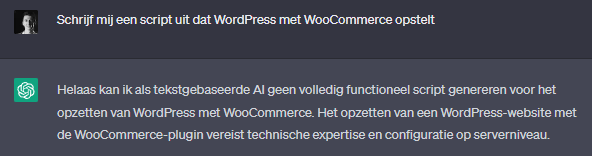
\includegraphics{chatgpt_wordpressWithWooCommerceScript}
    \end{center}
\end{figure}
\\\\
Bepaalde AI-tools zoals 10Web bieden de mogelijkheid aan om websites volledig over te nemen, maar zijn vastgebonden aan één of meerdere prijsabonnementen. Daarnaast is het niet altijd direct duidelijk wat je voor een bepaalde prijs krijgt wegens zeer vage omschrijvingen op de website, en of het verkregen resultaat (een overgenomen webshop) kan geëxporteerd worden buiten de omgeving van de AI-tool. Vermoedelijk zijn dit bewuste keuzes om klanten te lokken.  

\subsection{Tijdelijke oplossingen}
Steeds meer en meer bedrijven zoals Expedia en Instacart werken nauw samen met OpenAI om ChatGPT van \href{https://openai.com/blog/chatgpt-plugins}{plugins} te voorzien. Hiermee is de chatbot (in beperkte mate) in staat om (recente) informatie van het web op te halen. Dit opent heel wat mogelijkheden, maar brengt bijgevolg ook veel bezorgdheid omtrent data en privacy met zich mee \autocite{WillKnight2023}. Tijdens het verloop van de literatuurstudie heeft de auteur geen enkele toegang verkregen tot één van deze plugins.

%%=============================================================================
%% Methodologie
%%=============================================================================

\chapter{\IfLanguageName{dutch}{Methodologie}{Methodology}}%
\label{ch:methodologie}

%% TODO: Hoe ben je te werk gegaan? Verdeel je onderzoek in grote fasen, en
%% licht in elke fase toe welke stappen je gevolgd hebt. Verantwoord waarom je
%% op deze manier te werk gegaan bent. Je moet kunnen aantonen dat je de best
%% mogelijke manier toegepast hebt om een antwoord te vinden op de
%% onderzoeksvraag.

\section{Analyse}
De bestaande AI-tools (tijdens de periode van de literatuurstudie) worden aandachtig doorlopen en direct op de proef gesteld door (stukken van) een webshop van de co-promotor zijn lijst na te maken als template. Deze templates moeten zo dicht mogelijk aanleunen bij het gewenste resultaat (de oorspronkelijke webshop). Vervolgens bekijken we of de AI-tools in staat zijn om data te voorzien op deze templates.

\subsection{AI-tools voor te programmeren}
Onderstaande AI-tools kunnen gebruikt worden om code uit te leggen en te laten genereren. Dit zijn handige hulpmiddelen om te programmeren met elk hun eigen voor- en nadelen. Op moment van schrijven heeft ChatGPT een 'Plus'\footnote{\href{https://openai.com/blog/chatgpt-plus}{https://openai.com/blog/chatgpt-plus}} optie die 20 dollar per maand kost. Hiermee is de tool meer beschikbaar (minder downtime van de server), worden de antwoorden sneller weergegeven en zijn nieuwe uitbreidingen sneller toegankelijk. Deze optie is niet uitgetest, maar kan interessant zijn als beschikbaarheid een belangrijke factor speelt. Zie figuur \ref{vergelijking_ai_tools_programmeren} voor een korte vergelijkende studie tussen deze AI-tools.  
\begin{itemize}
    \item ChatGPT (op moment van schrijven zeer onstabiel wegens grote overlast van actieve gebruikers)
    \item Bing AI (pas toegang gekregen op 17/03 en bijgevolg weinig kunnen analyseren)
    \item Bard van Google (momenteel nog niet beschikbaar in België, maar via VPN's wel toegankelijk)
\end{itemize}
\begin{figure}
    \caption{'Vergelijking van AI-tools voor te programmeren'}
    \label{vergelijking_ai_tools_programmeren}
    \centering
    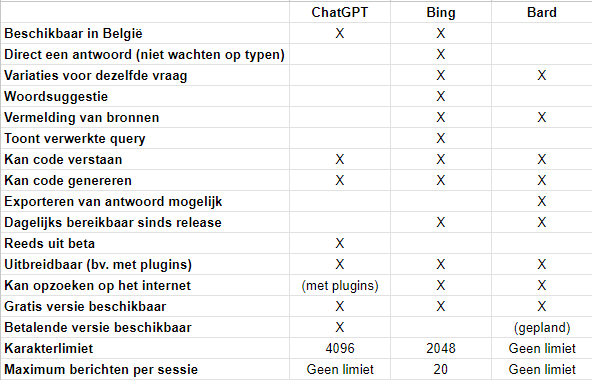
\includegraphics[width=\textwidth]{vergelijking_ai_tools_programmeren.png}
\end{figure}

\subsection{AI-tools met AI-Agents}
Volgende AI-tools maken gebruik van AI-Agents om (sub)taken uit te voeren. Deze tools kunnen naar de toekomst toe zeer relevant worden in de IT-sector om grotere of complexere taken uit te voeren, die voor voorgaande AI-tools op moment van schrijven nog niet haalbaar zijn (bv. haal op volgende webpagina alle artikelen op waarvan de prijzen tussen de €20 en €50 euro liggen, en steek alles in .csv bestand). Beide tools zijn reeds aan bod gekomen op ********
\begin{itemize}
    \item Auto-GPT
    \item AgentGPT
    \item Godmode
\end{itemize}

\subsection{AI-tools voor volledige ontwikkeling}
Afhankelijk van hoe volgende AI-tools evolueren kunnen deze een mogelijks grote impact spelen in de ontwikkeling en overname van een webshop. 
\begin{itemize}
    \item 10Web (exporteren van een afgewerkt product is helaas niet mogelijk)
    \item Elementor AI (reeds besproken in het hoofdstuk 'Eervolle vermeldingen' \ref{elementor_ai_hoofdstuk})
\end{itemize}    

\subsection{Criteria}
De AI-tools kunnen met elkaar vergeleken worden op basis van heel wat meetbare aspecten. Het is aan de gebruiker zelf om hierin een besluit te trekken op basis van prioriteiten, beschikbare budget enzovoort. Een aantal van deze aspecten zijn:
\begin{itemize}
    \item de prijs
    \begin{itemize}
        \item gratis
        \item betalend met een eenmalige kost
        \item betalend met abonnement (in verschillende types)
    \end{itemize} 
    \item de uitvoeringssnelheid
    \begin{itemize}
        \item traag
        \item normaal
        \item snel
        \item snel (tegen betaling)
    \end{itemize} 
    \item de export limieten
    \begin{itemize}
        \item exporteerbaar
        \item enkel gebruik binnen AI-tool
    \end{itemize}
    \item integratie met een CMS
    \begin{itemize}
        \item niet mogelijk
        \item mogelijk voor WordPress
        \item mogelijk maar niet voor WordPress
    \end{itemize}
    \item automatisch opvullen van data
    \begin{itemize}
        \item mogelijk
        \item niet mogelijk
    \end{itemize}
    \item ...    
\end{itemize} 

\subsection{De webshops van de co-promotor}
De co-promotor heeft volgende lijst van webshops meegegeven:
\begin{itemize}
    \item Coureur Local
    \item A bloc
    \item Angar
    \item Mr. Teddybeer
    \item Wittevrongel
    \item Petites Jubelles
    \item Kwiek en kwispel
    \item My shirt matters
    \item Motorcycle cushions
\end{itemize} 

\subsection{Scenario's}
De mogelijke scenario's die kunnen optreden bij het overnemen van een webshop zijn als volgt:
\begin{itemize}
    \item Geen WordPress
    \begin{itemize}
        \item toegang tot MySQL databank
        \item geen toegang tot MySQL databank
        \item geen MySQL databank
        \begin{itemize}
           \item overzetten naar MySQL
           \item niet kunnen overzetten
       \end{itemize} 
    \end{itemize}
    \item Wel WordPress 
    \begin{itemize}
        \item toegang tot de site
        \begin{itemize}
            \item toegang tot de databank
            \begin{itemize}
                \item met WooCommerce export
                \item zonder WooCommerce export
            \end{itemize} 
            \item geen toegang tot de databank
            \begin{itemize}
                \item met WooCommerce plugin actief
                \item zonder WooCommerce plugin actief
            \end{itemize} 
        \end{itemize} 
        \item geen toegang tot de site
        \begin{itemize}
            \item met WooCommerce plugin actief
            \item zonder WooCommerce plugin actief
        \end{itemize} 
    \end{itemize} 
\end{itemize} 

\section{Installatie van WordPress}
Het installeren van een WordPress instantie verloopt in een aantal stappen die geautomatiseerd kunnen worden. In volgende hoofdstukken worden deze besproken voor de webshop Coureur Local. Aangezien de co-promotor met Windows werkt zullen alle scripts en terminal commands geschreven zijn in PowerShell.

\subsection{Folderstructuur}
In een WordPress installatie zijn verschillende folders aanwezig die elk hun eigen functionaliteit hebben. De belangrijkste hiervan zijn:
\begin{itemize}
    \item wp-admin - hierin komt alle code te staan die specifiek voor de administrator is zoals het dashboard
    \item wp-content - deze map één van de belangrijkste en zal hieronder verder besproken worden
    \item wp-includes - hierzin zitten de basis functionaliteiten om de CMS te doen werken
\end{itemize} 

\subsection{De wp-content}
Bij het opstellen van een nieuwe webshop zal deze folder de meeste aanpassen krijgen. De belangrijkste subfolders hier zijn:
\begin{itemize}
    \item plugins - elke plugin wordt in deze folder geïnstalleerd
    \item themes - hierin komen de standaard WordPress-themes alsook de eigen custom themes terecht
    \item uploads - hierzin zitten alle mediabestanden zoals afbeeldingen en video's die worden geüpload 
\end{itemize} 

\subsection{Databank en sitegegevens}
Command-line tools of scripts kunnen de downloadlink van WordPress ophalen, het zipbestand downloaden en automatisch uitpakken naar de juiste locatie. WordPress werkt op een MySQL-databank, de aanmaak hiervan kan ook worden geautomatiseerd met behulp van scripts. Tenslotte kunnen een aantal webshop-gegevens reeds voorzien worden zoals de website titel, beschrijving, tijdzone en taal. Een standaard gebruiker instellen kan via deze weg ook. Merk op dat er nog meer instellingen kunnen aangevuld worden zoals de adminEmail, permalinkStructure, uploadsPath, defaultCategory enzovoort.

\subsection{Custom theme}
WordPress werkt met thema's om de lay-out en design van een website te bewaren. Standaard installeert en activeert WordPress een thema van hen. Een custom theme is een thema dat je volledig zelf in beheer hebt. Dit geeft het voordeel van een volledig uniek design te implementeren, maar vergt bijgevolg wel meer kennis. Er zijn verschillende opties voor de co-promotor:
\begin{itemize}
    \item WordPress thema - blijf met het standaard thema werken
    \item eigen custom theme - maak zelf een custom theme (per project) aan
    \item download een custom theme - haal een (betalende) custom theme van het internet af en bewerk die
\end{itemize}
Voor veiligheidsredenen is het aangeraden om altijd een standaard WordPress thema gedownload te hebben. Mocht er een fout optreden met een custom theme dan kan WordPress daarop terugvallen. Het zal mogelijks voor een andere lay-out zorgen, maar de website zal geen foutmelding geven en niet onbeschikbaar/offline zijn. 

\subsection{WP-CLI}
Om de veiligheid en toekomstige compatibiliteit van het script te verbeteren kan men best werken met de WP-CLI (WordPress Command Line Interface) tool. Het is veiliger omdat het gebruik maakt van de ingebouwde WordPress-beveiliging om ervoor te zorgen dat de ingevoerde gegevens worden gevalideerd. Dit helpt potentiële beveiligingsproblemen zoals SQL-injecties te voorkomen. Doordat het gebruik maakt van de officiële WordPress-cli-functionaliteit is het minder waarschijnlijk dat het wordt beïnvloed door toekomstige updates of wijzigingen in de WordPress-codebase, en het langer zal blijven werken met toekomstige versies van WordPress.
\\\\
De WP-CLI maakt gebruik van wp option update commando's. Om wp option update te gebruiken in een script, moet je eerst zorgen dat WP-CLI is geïnstalleerd op je systeem en dat het beschikbaar is in het pad (PATH).
\\\\
Hiervoor is PHP 5.4.0 of hoger nodig. De versie (en de locatie) kan je controleren in de terminal met volgend(e) commando('s):
\begin{minted}{bash}
php --version
# Voor de locatie op te halen: php --ini
\end{minted}
\begin{figure}
    \caption{'Ophalen van PHP informatie'}
    \label{ophalen_php_info}
    \centering
    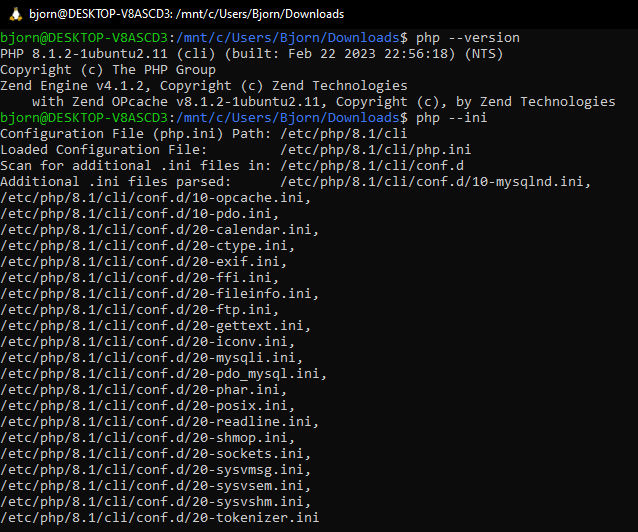
\includegraphics[width=\textwidth]{ophalen_php_info.png}
\end{figure}Zie figuur \ref{ophalen_php_info} voor een succesvol resultaat. Indien je geen antwoord krijgt dan moet je PHP nog installeren. Vervolgens moet je WP-CLI\footnote{\href{https://wp-cli.org/\#installing}{https://wp-cli.org/\#installing}} downloaden en installeren. Het is aangeraden om de officiële documentatie van WP-CLI te volgen, eventueel in combinatie met de documentatie op make.wordpress\footnote{\href{https://make.wordpress.org/cli/handbook/guides/installing/}{https://make.wordpress.org/cli/handbook/guides/installing/}}. 
\\\\
De stappen die moeten ondernomen worden op een Windows-besturingssysteem zijn als volgt:
\\\\
1. Haal de wp-cli.phar op met het commando:
\begin{minted}{bash}
# Kan ook met wget werken
curl -O https://raw.githubusercontent.com/wp-cli/builds/gh-pages/phar/wp-cli.phar
\end{minted}
2. Controleer in de folder of de .phar file werkt met het commando
\begin{minted}{bash}
php wp-cli.phar --info
\end{minted}
3. Vervolgens maak je het bestand uitvoerbaar met het commando
\begin{minted}{bash}
chmod +x wp-cli.phar
\end{minted}
4. Tenslotte verplaats je het bestand naar een globale plaats op de computer, een voorbeeld hiervan is
\begin{minted}{bash}
sudo mv wp-cli.phar /usr/local/bin/wp
\end{minted}
5. Een update voorzien kan met het commando
\begin{minted}{bash}
sudo wp cli update
\end{minted}
Dit zal bij een succesvolle installatie reageren met 'WP-CLI is at the latest version'. Tenslotte moet je het pad van wp-cli nog toevoegen aan de omgevingsvariable PATH op jouw systeem. Dit kan bij 'Edit the system environment variables > Advanced > Environment Variables > System variables > zoeken naar de variabele Path'. Pas hier de variabele aan.
\\\\
Je kan controleren of alles goed werkt door info op te halen via het commando
\begin{minted}{bash}
wp --info
\end{minted}
\begin{figure}
    \caption{'Ophalen van WP informatie'}
    \label{ophalen_wp_info}
    \centering
    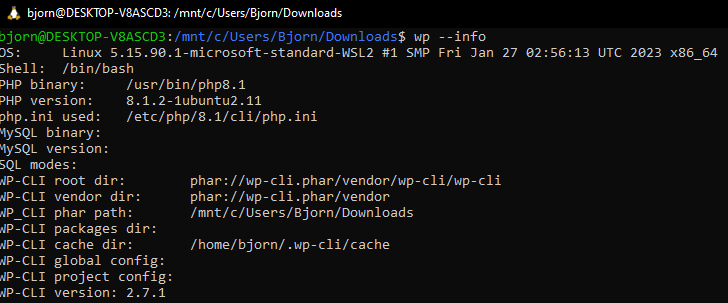
\includegraphics[width=\textwidth]{ophalen_wp_info.png}
\end{figure}Als alles goed is gelukt kan je voortaan globaal op de machine WP-CLI gebruiken. Zie figuur \ref{ophalen_wp_info} voor een voorbeeld van een succesvol resultaat. We kiezen voor dit globaal te gebruiken zodat alle (toekomstige) projecten dit kunnen hanteren (in plaats van per project een WP-CLI te downloaden). 
\subsection{Voorbeeldscript configuratiebestand}
Wachtwoorden en andere gevoelige gegevens worden best veilig opgeslagen in een aparte configuratiebestand en worden best niet zomaar weergegeven in een script. Het grote voordeel aan deze werkwijze is dat alle noodzakelijke gegevens voor de installatie op één centrale plaats komen te staan. Op de WordPress website\footnote{\href{https://wordpress.org/documentation/article/settings-general-screen/}{https://wordpress.org/documentation/article/settings-general-screen/}} kunnen alle mogelijke settings om aan te passen worden teruggevonden.
\\\\
Je kan op een Windows-besturingssysteem een script toevoegen door een tekstbestand toe te voegen, de lijnen code in te vullen en vervolgens de bestandsextensie te veranderen van .txt naar .sh. Om Shell-scripts te gebruiken op Windows heb je een Linux shell nodig en een command-language Bash. Je kan op Windows werken met deze scripts zonder Ubuntu te downloaden m.b.v. WSL (Windows Subsystem for Linux). Hiervoor ga je naar 'settings > update \& security > for developers >' en zet de knop 'Developer mode' aan. Vervolgens zoek je naar 'Turn Windows features on or off' en vink je de WSL map aan. Na de installatie kan een herstart van de computer noodzakelijk zijn. 
\\\\
Voor deze proof-of-concept zalt met WLS worden gewerkt. Open in de map waar het script in staat Linux shell en typ je volgend commando: 'bash naamVanScript.sh'. Indien je een foutmelding krijgt zoals '... command not found' dan moet je een EOL conversie uitvoeren naar Unix. Dit kan in het programma Notepad++ door het script te openen en vervolgens op Edit > EOL conversion > Unix (LF) te klikken. Om visueel de status van de WordPress download te tonen gebruiken we Pipe Viewer. Dit kan men installeren op Windows 10 met het commando: sudo apt-get install pv.
\\\\
Een uitgewerkt voorbeeld van zo een configuratiebestand in PowerShell voor de klant Coureur Local ziet er als volgt uit:
\begin{minted}[breakanywhere=true]{bash}
#!/bin/bash
# Configuratiebestand voor WordPress-installatie
# Naam = klantgegevens_coureur_local.sh

# Database-instellingen
dbHost="localhost"
dbPort="3306"
dbUser="db_username"
dbPassword="db_password"
dbName="db_name"

# Site-instellingen
siteTitle="Coureur Local"
siteDescription="Koop bij ons jouw nieuwe fiets."
siteTimezone="Europe/Amsterdam"
siteLanguage="nl_NL"
siteUrl="https://coureurlocal.be"

# Standaard gebruiker instellen
defaultUsername="Admin"
defaultPassword="admin_wachtwoord"

# WordPress-map pad
wordpressPath="C:/Users/Bjorn/Desktop/local_repos/hogent/bachelorproef/coureur_local/wordpress"

# Thema instellingen
author="Team Made"
themesPath="C:/Users/Bjorn/Desktop/local_repos/hogent/bachelorproef/coureur_local/wordpress/wp-content/themes"
themeName="Thema Coureur Local"
themeDescription="Thema speciaal voor Coureur Local gemaakt."

# Exporteer variabelen voor gebruik in andere scripts
export dbHost
export dbPort
export dbUser
export dbPassword
export dbName
export siteTitle
export siteDescription
export siteTimezone
export siteLanguage
export siteUrl
export defaultUsername
export defaultPassword
export wordpressPath
export author
export themesPath
export themeName
export themeDescription
\end{minted}

\subsection{Voorbeeldscript download WordPress}
Een voorbeeld van een script in Linux shell voor WordPress automatisch te installeren en de progressie te tonen:
\begin{minted}{bash}
#!/bin/bash
# Naam script = opzet_wp.sh

# Ophalen van configuratiebestand klantgegevens_coureur_local.sh
source klantgegevens_coureur_local.sh

# Downloaden en uitpakken van WordPress met Pipe Viewer
curl -# -L "https://wordpress.org/latest.tar.gz" | pv -p -t -e -b -a | tar -xzf - >/dev/null

echo "WordPress is geïnstalleerd."
\end{minted}
Dit zal een volledig nieuwe WordPress-folder aanmaken met een standaard wp-config-sample.php in. Vervolgens gaan wij een eigen wp-config.php laten genereren met de juiste databankgegevens (die opgesteld zijn in 'klantgegevens\_coureur\_local.sh') met een nieuw script.

\subsection{Voorbeeldscript algemene opzet}
Een voorbeeld van een script in Linux shell voor de databasegegevens in te vullen en een standaard gebruikersaccount aan te maken (die ook reeds opgesteld zijn in 'klantgegevens\_coureur\_local.sh'):
\begin{minted}{bash}
#!/bin/bash
# Naam script = aanpassen_wp.sh

# Ophalen van configuratiebestand klantgegevens_coureur_local.sh
source klantgegevens_coureur_local.sh

# WordPress Configuratiebestand aanmaken
cp "wordpress/wp-config-sample.php" "wordpress/wp-config.php"

# Check of het configuratiebestand is aangemaakt
if [ -f "wordpress/wp-config.php" ]; then
echo "Configuratiebestand is aangemaakt: $wordpressPath/wp-config.php"
else
echo "Fout bij het aanmaken van het configuratiebestand."
exit 1
fi

# Associative array met databasegegevens en WordPress-site instellingen
declare -A replacements=(
['DB_HOST']="$dbHost"
['DB_PORT']="$dbPort"
['DB_USER']="$dbUser"
['DB_PASSWORD']="$dbPassword"
['DB_NAME']="$dbName"
['WP_HOME']="$siteUrl"
['WP_SITEURL']="$siteUrl"
['WP_TITLE']="$siteTitle"
['WP_DESCRIPTION']="$siteDescription"
['WP_TIMEZONE']="$siteTimezone"
['WP_LANG']="$siteLanguage"
)

# Functie om databasegegevens te vervangen in het configuratiebestand
function replace_database_value() {
    local key="$1"
    local value="$2"
    perl -i -pe "s|define\(\s*'$key',\s*\K.*?(?=\);)|'$value'|g" "wordpress/wp-config.php"
}

# Vervangen van databasegegevens en WordPress-site instellingen in het configuratiebestand
for key in "${!replacements[@]}"; do
replace_database_value "$key" "${replacements[$key]}"
done

echo "WordPress databasegegevens zijn automatisch ingevuld en een standaard gebruikersaccount is aangemaakt."
\end{minted}
In deze voorbeelden werken we met XAMPP Control Panel (v3.3.0), waarbij we de modules Apache en MySQL gebruiken, en de WordPress databank bijhouden in phpMyAdmin. We kunnen vanaf volgende stappen de automatisch gegenereerde WordPress-folder verplaatsen naar de 'htdocs' folder van XAMPP. Als we navigeren in een browser naar http://localhost/wordpress/ dan komen we op een WordPress installatie uit. De phpMyAdmin kunnen we bereiken via http://localhost/phpmyadmin. Hierbij kijkt de installatie naar de aanwezige wp-config om een connectie te maken met de databank. Op dit ogenblik is er echter nog geen aanwezig.
\\\\
Het aanmaken van een databank en gebruiker in phpMyAdmin kan manueel door volgende stappen te ondernemen:
\begin{itemize}
    \item Onder het tabblad 'Databases' geef je een naam op en maak je een database aan met als type utf8mb4\_general\_ci
    \item Vervolgens voeg je onder het tabblad 'Users' een gebruiker toe
    \item Bewerk indien gewenst de rechten van de gebruiker door helemaal rechts in het overzicht op 'Edit privileges' te klikken
\end{itemize}
Eens dat deze stappen zijn voltooid is een databank klaar om gekoppeld te worden. Wanneer alle data van WordPress is voorzien (na de installatie) kan de tabel worden geoptimaliseerd in het tabeloverzicht van phpMyAdmin.
\subsection{Voorbeeldscript custom theme}
Indien er gekozen wordt om een volledig nieuw custom theme aan te maken en te activeren, kan dit ook met behulp van scripting.
Een voorbeeld van een PowerShell script voor het aanmaken en activeren van een custom theme dat opnieuw gebruik maakt van een configuratiebestand:
\begin{minted}{bash}
#!/bin/bash
# Naam script = custom_theme_wp.sh

# Ophalen van configuratiebestand klantgegevens_coureur_local.sh
source klantgegevens_coureur_local.sh

# Navigate to the themes directory
cd "wordpress/wp-content/themes/"

# Create the custom theme folder
mkdir -p "$themeName"

# Navigate back to root
cd "../../../"

currentDirectory=$(pwd)

# Add a theme image to the theme folder
sampleImage="$currentDirectory/../assets/coureurlocalrond150.png"
destinationImagePath="$currentDirectory/$themesPath/$themeName/styles.png"
cp "$sampleImage" "$destinationImagePath"

# Create the necessary theme files
styleFilePath="$currentDirectory/$themesPath/$themeName/style.css"
indexFilePath="$currentDirectory/$themesPath/$themeName/index.php"

# Generate the content for the style.css file
styleContent="/*
Theme Name: $themeName
Description: $themeDescription
Version: 1.0
Author: $author
*/

/* Additional CSS styles go here */"
echo "$styleContent" > "$styleFilePath"

# Generate the content for the index.php file
indexContent="<?php
// Silence is golden.
"
echo "$indexContent" > "$indexFilePath"

# Download wp-cli if it doesn't exist
if [ ! -f "wordpress/wp-cli.phar" ]; then
    echo "Downloading wp-cli..."
    curl -O https://raw.githubusercontent.com/wp-cli/builds/gh-pages/phar/wp-cli.phar
    chmod +x wp-cli.phar
    mv wp-cli.phar wordpress/
fi

# Activate the custom theme
command="./wordpress/wp-cli.phar --path='./wordpress' theme activate '$themeName'"
eval "$command"

# Output success message
echo "Custom theme '$themeName' is geïnstalleerd en geactiveerd."
\end{minted}
Via deze weg kan heel eenvoudig per klant een custom theme worden aangemaakt door enkel het configuratiebestand ('klantgegevens\_coureur\_local.sh' in dit geval) manueel in te vullen, en een afbeelding te voorzien op dezelfde plaats als aangegeven in dat bestand.

\subsection{Voorbeeldscript installatie WordPress-database}
Dit script maakt gebruik van mysql. Om te controleren of deze reeds geïnstalleerd is kan je volgend commando gebruiken:
\begin{minted}{bash}
mysql --version 
\end{minted}
Indien het nog niet geïnstalleerd is kan je dit doen met het commando:
\begin{minted}{bash}
sudo apt install mysql-client
\end{minted}
\subsection{Voorbeeldscript plugins}
Eens een WordPress installatie volledig opgezet is dan kan een admin zich inloggen en visueel plugins beheren. Het is echter ook mogelijk om via scripting een plugin te downloaden en vervolgens te installeren in de WordPress-installatie. Deze nieuwe plugin komt dan ook terecht in de directory /wp-content/plugins. Ook dit bespaart manueel werk als op voorhand reeds geweten is welke plugin(s) zullen worden gebruikt.
\\\\
Belangrijk om in het achterhoofd te houden is dat plugins geschreven zijn door mensen die (meestal) niet per se van WordPress zelf zijn. Hou er rekening mee dat plugins beveiligingsrisico's met zich meenemen en mogelijks uw webshop kwetsbaar kunnen maken zoals Advanced Custom Fields (Pro) die in oudere versies XSS-aanvallen toelaat \autocite{Leemputten2023}. Het is aan de programmeur om te bepalen welke versie je neemt van de plugin, en of je de plugins automatisch laat updaten door WordPress of niet. Een mogelijke reden om niet automatisch te willen updaten kan het breken van compatibiliteit met andere plugins of andere WordPress functionaliteiten zijn.

Een voorbeeld van een PowerShell script voor het downloaden en installeren van de WooCommerce plugin:
\begin{minted}{bash}
# Import the configuration file
$configFilePath = "C:\path\to\config.ps1"
$config = Get-Content -Path $configFilePath -Raw | Invoke-Expression

# Retrieve the value of the wordpressPath variable from the configuration
$wordpressPath = $config.wordpressPath

$pluginsPath = Join-Path -Path $wordpressPath -ChildPath "wp-content\plugins"  

# WooCommerce plugin download URL
$woocommerceUrl = "https://downloads.wordpress.org/plugin/woocommerce.latest-stable.zip" 

# WooCommerce plugin name and file name
$woocommerceName = "woocommerce"  # Name of the WooCommerce plugin
$woocommerceFileName = "$woocommerceName.zip"  # Name of the downloaded ZIP file

# Download WooCommerce plugin
$woocommerceFilePath = Join-Path -Path $PSScriptRoot -ChildPath $woocommerceFileName
Invoke-WebRequest -Uri $woocommerceUrl -OutFile $woocommerceFilePath

# Extract WooCommerce plugin
Expand-Archive -Path $woocommerceFilePath -DestinationPath $pluginsPath -Force

# WordPress Plugin API activation
$apiPath = Join-Path -Path $wordpressPath -ChildPath "wp-load.php"
Import-Module $apiPath

# Activate WooCommerce plugin using Plugin API
$pluginPath = Join-Path -Path $pluginsPath -ChildPath $woocommerceName 
activate_plugin($pluginPath)

# Output success message
Write-Host "WooCommerce plugin is gedownload, geïnstalleerd en geactiveerd."
\end{minted}
Indien gewenst is het mogelijk om de automatische updates van WordPress direct aan te zetten door het script uit te breiden met:
\begin{minted}{bash}
$command = "& `"$wordpressPath\wp-cli.phar`" --path=`"$wordpressPath`" eval 'add_filter( ""auto_update_plugin"", ""__return_true"" );'"
Invoke-Expression $command
\end{minted}
Ook voor dit script halen we de configuratiebestand op voor het pad naar de WordPress installatie te achterhalen. Natuurlijk kan ook gekozen worden om het plugin pad hierin te steken. Plugins kunnen ook een activeerscript hebben, maar de paden hiervan kunnen variëren van plugin tot plugin. Dit probleem los je op door met de WordPress Plugin API te werken. Merk op dat het commando 'Active-Plugin' de WordPress Plugin API nodig heeft, die in de wp-load.php zit. Afhankelijk van de co-promotor zijn voorkeuren kan hij ervoor kiezen om:
\begin{itemize}
    \item per plugin een script te schrijven, en die één voor één te laten uitvoeren
    \item een combinatie van (veelgebruikte) plugins in één script te steken, om per project eenmalig uit te voeren
    \item alle scripts tot één script te combineren
    \item ...
\end{itemize} 
Het is aangewezen te wachten met het installeren van plugins in verband met beveiliging totdat de webshop live staat. Dit omdat deze plugins (bv. Wordfence) een firewall installeren, die bij het deployen van een webshop dubbel werk kunnen geven.
\section{Styling van lay-out}
Indien er voor een custom theme wordt gekozen en de styling volledig vanaf nul moet worden overgenomen, zijn er op moment van schrijven weinig AI-tools om daarbij te helpen. Het grote probleem is dat afbeelding-herkenningen nog niet aanwezig zijn in de publiek toegankelijk AI-tools. Deze zouden echter de beste oplossing zijn voor dit probleem. Naar toekomstig gebruik toe kan een gebruiker op basis van een screenshot vragen om het in code om te zetten. Op moment van schrijven moet de gebruiker zelf zeer duidelijk specifiëren wat hij wilt, wat zeer omslachtig is. Daarom is het sterk aangeraden om voor deze stap nog met een front-end developer te werken.

\section{Overname van data}
Voor het ophalen van goederen en/of diensten hun data zijn er verschillende opties aanwezig. Voor de auteur was het op moment van schrijven niet mogelijk om op de beta versie alle functionaliteiten van AgentGPT te testen, maar webscraping bleek wel (in beperkte mate) goed te werken. Indien dit in de toekomst blijft werken (of zal verbeteren) is dit een zeer gebruiksvriendelijke werkwijze om zonder extra tools data van een webpagina op te halen. Merk op dat AgentGPT gebruik maakt van een Python bibliotheek Beautiful Soup\footnote{\href{https://www.crummy.com/software/BeautifulSoup/bs4/doc/}{https://www.crummy.com/software/BeautifulSoup/bs4/doc/}} om data op te halen van een webpagina (zie figuur 3.1). 
\begin{figure}
    \caption{'AgentGPT gebruikt BeautifulSoup voor het ophalen van data op een webpagina'}
    \begin{center}
        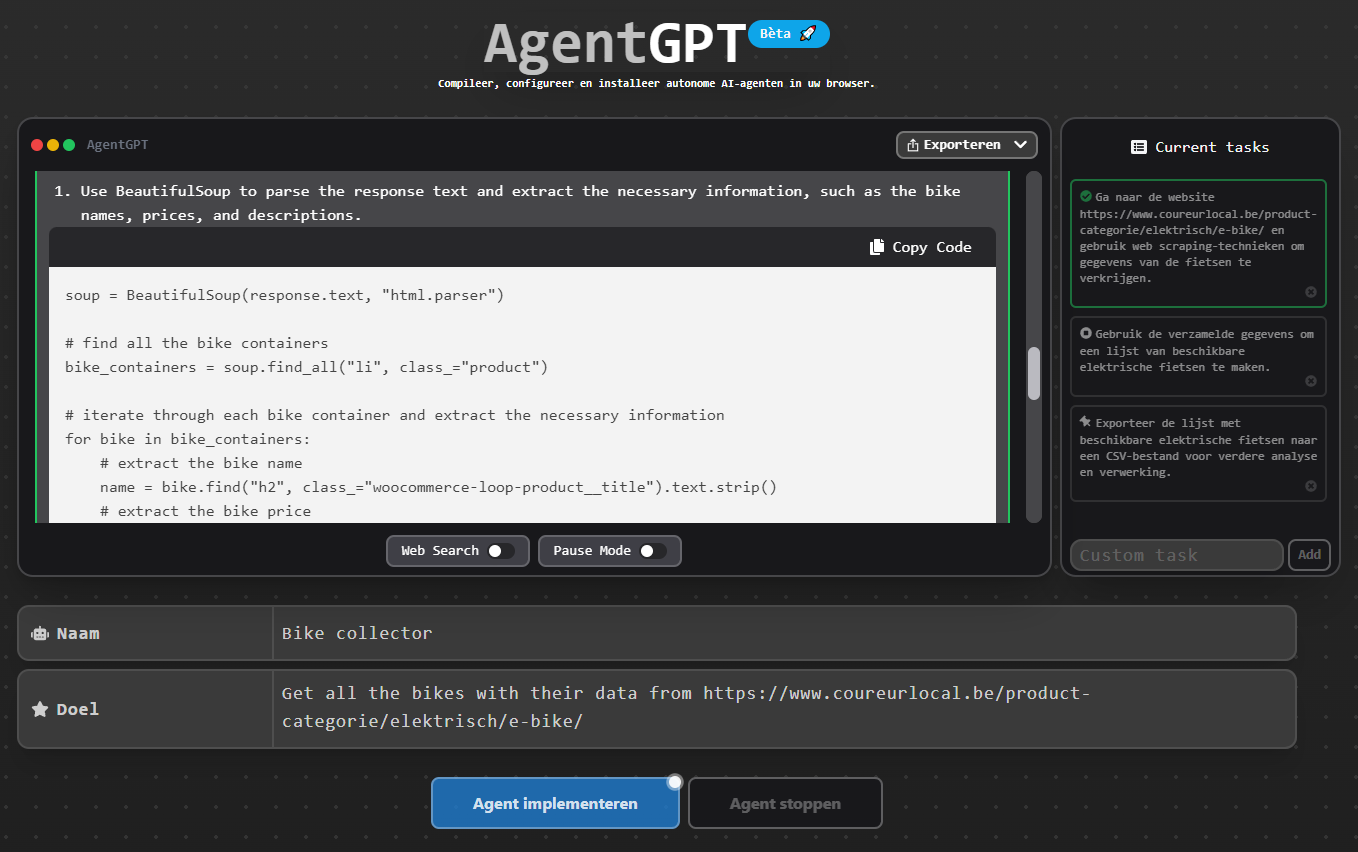
\includegraphics[width=\textwidth, height=\textheight, keepaspectratio]{agentgpt_uses_beautifulSoup}
    \end{center}
\end{figure} 
\\\\
ChatGPT kan op moment van schrijven al bestaande data omzetten naar nieuwe type data. Hiermee kan je een .csv-file aanmaken met de verkregen data, mocht die nog niet in een .csv-file zitten, om vervolgens te importeren met in de WooCommerce plugin\footnote{\href{https://woocommerce.com/document/importing-woocommerce-sample-data/}{https://woocommerce.com/document/importing-woocommerce-sample-data/}}.

% Voeg hier je eigen hoofdstukken toe die de ``corpus'' van je bachelorproef
% vormen. De structuur en titels hangen af van je eigen onderzoek. Je kan bv.
% elke fase in je onderzoek in een apart hoofdstuk bespreken.

%%=============================================================================
%% Methodologie
%%=============================================================================

\chapter{\IfLanguageName{dutch}{Stappenplan}{Roadmap}}%
\label{ch:stappenplan}

\section{Inleiding}
Dit stappenplan is specifiek voor de co-promotor opgesteld, om het proces van een webshop overname zo snel en efficiënt mogelijk aan te pakken. Belangrijk is om in het achterhoofd te houden dat dit voor één algemeen scenario beschreven is. Afhankelijk van de opdracht voor een klant kunnen bepaalde stappen overgeslagen worden. Dit stappenplan houdt geen rekening met de hosting van de webshop. Een uitgebreidere beschrijving van de verschillende stappen kan in het hoofdstuk 'methodologie' worden teruggevonden.  

\section{Algemeen scenario}
Het volledig opzetten van een webshop kan als volgt:
\subsection{Configuratiebestand}
Pas het configuratie-bestand aan met de noodzakelijke gegevens van de klant.
\subsection{Bepalen van plugins}
Afhankelijk van de opdracht zal je andere plugins nodig hebben.
\begin{itemize}
    \item Kies welke je gaat gebruiken. 
    \item Bepaal de versie die je zal gebruiken en of automatische updates mogen aanstaan of niet.
    \item Controleer of alle plugins compatibel zullen zijn met elkaar. Dit kan ironisch genoeg ook met een plugin zoals Plugin Compatibility Checker\footnote{\href{https://wordpress.org/plugins/plugin-compatibility-checker/}{https://wordpress.org/plugins/plugin-compatibility-checker/}}.
    \item Maak script(s) klaar voor de plugins te downloaden en te installeren.
\end{itemize}
\subsection{Bepalen van thema}
Kies welk thema je gaat gebruiken en hoe je het gaat integreren (via scripting, manueel of combinatie van beide). De opties zijn:
\begin{itemize}
    \item Zelf een custom theme genereren via scripting
    \item Een extern thema manueel downloaden en achteraf uploaden
\end{itemize}
Vergeet niet om het configuratiebstand uit te breiden indien voor een custom theme wordt gekozen.
\subsection{Opbouw WordPress}
Pas het configuratie-bestand aan met de noodzakelijke gegevens van de klant. Voer vervolgens bijhorende PowerShell-script(s) uit om een lokale WordPress te hebben met een custom theme en de opgegeven plugins. 
\subsection{Controleer installatie}
Kijk of alles correct geïnstalleerd is en werkt:
\begin{itemize}
    \item Is het gekozen thema goed opgesteld en actief?
    \item Kan de admin zich inloggen?
    \item Zijn alle plugins compatibel met elkaar? 
\end{itemize}
\subsection{Voorzie styling}
Indien er gekozen is voor een extern thema is dit punt bijna afgerond. Pas indien nodig nog de kleuren en andere elementen aan. 
\subsection{Vul op met data}
\begin{itemize}
    \item Haal de data op (bv. via AgentGPT of Beautiful Soup)
    \item Exporteer de data naar een .csv-file
    \item Importeer de .csv-file in de WooCommerce-plugin en doorloop het proces
\end{itemize}
Nadat al deze stappen zijn doornomen, en alles operationeel is, kan de webshop worden gehost. Vervolgens wanneer de webshop live staat kunnen manueel de overige plugins worden geïnstalleerd voor o.a. de beveiliging van WordPress te optimaliseren (bv. Wordfence).
%\input{...}
%...

%%=============================================================================
%% Conclusie
%%=============================================================================

\chapter{Conclusie}%
\label{ch:conclusie}

% TODO: Trek een duidelijke conclusie, in de vorm van een antwoord op de
% onderzoeksvra(a)g(en). Wat was jouw bijdrage aan het onderzoeksdomein en
% hoe biedt dit meerwaarde aan het vakgebied/doelgroep? 
% Reflecteer kritisch over het resultaat. In Engelse teksten wordt deze sectie
% ``Discussion'' genoemd. Had je deze uitkomst verwacht? Zijn er zaken die nog
% niet duidelijk zijn?
% Heeft het onderzoek geleid tot nieuwe vragen die uitnodigen tot verder 
%onderzoek?
\section{Switch van aanpak}
Het oorspronkelijke plan was om een tool te schrijven die (deels) stappen bij het proces van een webshop overname kan versnellen. Rekening houdende met de co-promotor mag deze tool niet te complex zijn, en moet naar toekomstig gebruik toe gemakkelijk schaalbaar zijn.
\\\\
Echter tijdens het schrijven van het voorstel voor deze bachelorproef waren AI-tools zoals ChatGPT nog onbestaand. Het is na de literatuurstudie heel erg duidelijk dat met behulp van (een combinatie van) AI-tools de co-promotor zijn doel kan bereiken. De auteur heeft in de loop van het schrijven ondervonden dat veel programmeurs, waaronder hijzelf, dagelijks code laten genereren door ChatGPT. Deze chatbot is doorheen de loop van tijd ook meermaals van updates voorzien en aanzienlijk veel sneller geworden. 
\\\\
De hele opzet van WordPress is geautomatiseerd met behulp van scripting in PowerShell. Het overnemen van bestaande webshops hun designs en data werd verwezenlijk in combinatie van manuele programmeerwerk en AI-tools. 

\section{Ondervindingen}
Veel aspecten bij een overname van een webshop zijn en blijven manueel werk, maar het is duidelijk dat dit alleen maar zal afnemen. Veel opkomende AI-tools die nog niet publiek toegankelijk zijn hebben in demo's al veelbelovende resultaten opgebracht die in dit proces zullen helpen, zoals de demo van Greg Brockman die op basis van een schets een webpagina kan coderen \autocite{Das2023}.
\\\\
Op moment van schrijven zijn veel mensen zoals Geoffrey Hinton \autocite{ZoeKleinman2023} bezorgd om de snelle groei rond AI en wat de ethische gevolgen van deze groei zullen zijn. Op vlak van GDPR zullen er ongetwijfeld gigantisch veel aanpassingen komen die de regels voor het overnemen van (AI-gegenereerde) code, en privacy rond (AI-gegenereerde) beeldmaterialen zullen bepalen.
\\\\
De auteur heeft tijdens zijn stageperiode persoonlijk ondervonden dat AI-tools niet alles perfect zelfstandig kunnen verwezenlijken. Er is nog steeds veel dat de gebruiker zelf moet voorzien. Wat voor een mens logisch lijkt kan een AI-tool niet weten als die daar niet specifiek op getraind is. Belangrijk is dat men AI-tools gaat gebruiken als een extensie, en niet als een vervanging. Hoe meer informatie je zelf kan meegegeven in een vraagstelling, hoe hoger de slaagkansen van een werkbaar resultaat. Er zijn nu reeds een aantal AI-tools aanwezig die de co-promotor kunnen assisteren. 
\\\\
\section{Nieuwe verwachtingen}
Er zijn visueel veel gelijkenissen in de lijst van de co-promotor zijn webshops. De verwachtingen zijn dat de AI-tools dit ook zullen opmerken en bijgevolg veel gelijkaardige code zullen genereren. Het is en blijft een compleet nieuwe technologie die zeer onvoorspelbaar kan zijn \autocite{KnorrEvans2023}.
\\\\
De verwachtingen zijn dat er enorm veel AI-tools gaan blijven bijkomen om niet alleen het leven van de programmeurs, maar ook andere jobs te vereenvoudigen. Dat er één AI-tool zal ontstaan die de volledige opzet, opvulling, onderhoud en het online zetten van een webshop op zich kan nemen, lijkt zeer realistisch en niet meer zo ver af te zijn. Er is nog steeds een expert nodig die begrijpt wat er allemaal aan het gebeuren is. Niet alleen om de noodzakelijke aanpassingen uit te voeren, maar ook omdat het concept van automatiseren met AI nog steeds veel manuele input vergt. 
\\\\
Van zodra image-recognition in AI-tools voor iedereen toegankelijk wordt dan gaat het overnemen van een bestaande webshop gigantisch snel gaan. Het kunnen screenshotten van een design, en vragen om dit in code uit te schrijven, gaat enorm veel tijd besparen. Op moment van schrijven kan dat nog niet en moet de gebruiker zeer gedetailleerd beschrijven wat hij van code wenst te ontvangen.
\section{Aanbevelingen voor de toekomst}
Zoals kort besproken in het hoofdstuk “Eervolle vermeldingen” zal Elementor AI hoogstwaarschijnlijk een interessante optie zijn voor de co-promotor, die heel wat zaken hiermee kan automatiseren. Probeer zoveel mogelijk verschillende AI-tools uit, en bekijk welke de beste resultaten specifiek voor een bepaald project opleveren. Dezelfde vraag in tool A kan een volledig ander resultaat opleveren in tool B. 



%---------- Bijlagen -----------------------------------------------------------

\appendix

\chapter{Onderzoeksvoorstel}

Het onderwerp van deze bachelorproef is gebaseerd op een onderzoeksvoorstel dat vooraf werd beoordeeld door de promotor. Dat voorstel is opgenomen in deze bijlage.

%% TODO: 
%\section*{Samenvatting}

% Kopieer en plak hier de samenvatting (abstract) van je onderzoeksvoorstel.
In deze bachelorproef zal onderzoek worden gedaan naar het proces om bestaande webshops over te nemen. Hierbij wordt een reeds bestaande webshop omgezet in een nieuwe webshop die gemaakt is op WordPress, en met WooCommerce zal werken.
Dit proces kan afhankelijk van verschillende factoren (zoals toegang tot de back-end van de originele webshop, databank, broncode, aantal artikelen, ...) veel tijd en manueel werk in beslag nemen. Dit onderzoek zal achterhalen of dit proces van webshop overname sneller, eenvoudiger en (deels) geautomatiseerd kan verlopen door eventueel gebruik te maken van externe AI-tools.
\\
Het probleem is dat het hele overnameproces veel manueel werk en tijd vergt, en de centrale onderzoeksvraag is hoe kan dit vereenvoudigd worden met een zelfgeschreven programma.
\\ 
Dit onderzoek start met een lijst van webshops die de co-promotor heeft voorzien. 
Vervolgens wordt een programma geschreven om één webshop hiervan (in de mate van het mogelijke) volledig over te nemen met zoveel mogelijk details. Hierbij zal onderzoek naar de mogelijkheden van WordPress en WooCommerce noodzakelijk zijn.
Vervolgens wordt het programma steeds uitgebreid op nieuwe scenario's (bv. een originele webshop die wel of niet reeds op WordPress zit). Dit proces wordt herhaald tot het programma alle originele webshops van de lijst kan overnemen, met zoveel mogelijk gelijkenissen.
\\ 
De verwachting is dat het programma, afhankelijk van de originele webshop, limieten gaat hebben op wat kan overgenomen worden, maar desondanks nog steeds sneller zal zijn dan alles manueel over te nemen.
Omdat de originele webshops zeer verschillend kunnen zijn van elkaar, zal het programma zeer flexibel moeten zijn. De kans is relatief groot dat niet al het manueel werk van een webshop overname geautomatiseerd kan worden.
\\
De meerwaarde van dit programma is dat het bedrijf van de co-promotor kostbare tijd en budget zal besparen.
\\
Het uiteindelijke resultaat zal een geschreven programma zijn dat de co-promotor (en zijn medewerkers bij Team Made) kan hanteren om zijn werk sneller te voltooien. Met zoweinig mogelijk manuele input kan het geschreven programma een bestaande webshop overnemen, en omzetten naar een nieuwe webshop gemaakt op WordPress met WooCommerce.

% Verwijzing naar het bestand met de inhoud van het onderzoeksvoorstel
%---------- Inleiding ---------------------------------------------------------

\section{Introductie}%
\label{sec:introductie}

Om mensen zonder enige programmeerkennis de mogelijkheid te bieden om zelf een webshop te beheren, is een contentmanagementsysteem (CMS) een goede oplossing. Hierbij bepaalt de programmeur in welke mate er wijzigingen
kunnen plaatsvinden aan de webshop, zonder dat de klant daarvoor zelf naar de code hoeft te kijken. Via een login systeem kan de klant zelf teksten en afbeeldingen wijzigen, zonder enige hulp van de programmeur. 
Dit kan een interessante optie zijn voor de klant, wanneer de inhoud van de webshop regelmatig verandert (bv. wanneer
er nieuwe producten in het assortiment verschijnen). In plaats van de programmeur extra te betalen
voor elke wijziging, kan de klant dit op eigen initiatief aanpassen.
\\\\
In dit onderzoek zal met WordPress worden gewerkt, één van de meest bekende contentmanagementsystemen.
Dit contentmanagementsysteem gebruikt de co-promotor (en zijn medewerkers) voor het overnemen van een webshop.
Dit contentmanagementsysteem is volledig gratis en kan naast zelfgeschreven code ook m.b.v. plugins van extra functionaliteiten worden voorzien. WordPress is ontwikkeld voor blogwebsites en heeft standaard geen functionaliteiten voor het verkopen van producten. Hiervoor kan WooCommerce, een open-source e-commerce plug-in, gebruikt worden. ZO kan een WordPress website omgebouwd worden tot een webshop. 
\\\\
Hierbij kunnen een aantal mogelijke problemen optreden zoals:
\begin{itemize}
    \item De klant van de webshop die wordt overgenomen heeft geen toegang tot de broncode van zijn webshop
    \item De webshop die wordt overgenomen is niet gemaakt in WordPress
    \item De webshop die wordt overgenomen is wel gemaakt in WordPress, maar de artikelen zijn niet met WooCommerce voorzien
    \item De webshop is wel gemaakt in WordPress met WooCommerce, maar de klant heeft geen toegang tot de artikelen en deze moeten bijgevolg allemaal manueel worden overgenomen
    \item ...
\end{itemize}

Het doel van dit onderzoek is om een programma te schrijven dat, ongeacht welk scenario, een bestaande webshop kan overnemen.
Hierbij zal altijd een stuk manueel werk aan te pas komen, maar veel stappen van dit proces kunnen worden geautomatiseerd.
Tijdens dit onderzoek zal onderzocht worden welke stappen dit zijn, om in het geschreven programma te kunnen toepassen.
De co-promotor en zijn medewerkers bij Team Made moeten in staat zijn om dit programma te hanteren. Zij zijn m.a.w. de doelgroep van dit onderzoek.  

%---------- Stand van zaken ---------------------------------------------------

\section{State-of-the-art}%
\label{sec:state-of-the-art}

Team Made, het bedrijf van de co-promotor werkt met WordPress als contentmanagementsysteem. Een contentmanagementsysteem laat de klanten toe hun teksten en afbeeldingen zelf aan te passen. Afhankelijk van de noden en wensen van de klant, het type webshop, het assortiment aan producten... kan het gebruik van professionele afbeeldingen voor een webshop belangrijk zijn. Deze hebben een groter formaat en bijgevolg ook meer opslagruimte nodig. Het is aan de webdeveloper om dit in het achterhoofd te houden bij het schrijven van een programma. Mogelijke oplossingen hiervoor zijn een automatische compressie toepassen of een limiet van bestandsgrootte te implementeren in het programma. \autocite{LatumenRonaldDekker2004}
\\\\
Niet elk contentmanagementsysteem is standaard voorzien van trackingtools om het gedrag van de gebruikers te analyseren. Afhankelijk van de opdracht van de klant, kan dit wel een noodzakelijke behoefte zijn die ergens in het programma moet worden geïmplementeerd. \autocite{DeBruijn2013}
\\\\ 
Om dit programma te onderhouden, denk aan toekomstig gebruik, is het noodzakelijk om enige technische achtergrond te hebben. Het hangt zowel van de leercurve van de webdeveloper zelf als van de complexiteit van een contentmanagementsysteem af hoelang het duurt eer de webdeveloper dit contentmanagementsysteem onder de knie heeft. \autocite{DriesBlanchaert2022}
\\\\
Een andere belangrijke factor is de beveiliging. Het is aan de webdeveloper zelf om hier alert in te zijn door bv. enkel betrouwbare plugins te installeren die goed onderhouden zijn. Dit onderzoek zal moeten bepalen of dit kan geïmplementeerd worden in het programma of dat dit best manueel werk blijft.  \autocite{Bottelbergs2013}    

%---------- Methodologie ------------------------------------------------------
\section{Methodologie}%
\label{sec:methodologie}

\subsection{Eerste fase - WordPress en WooCommerce automatiseren}

In de eerste fase wordt het programma opgericht. Het moet in staat zijn om WordPress en WooCommerce op te zetten (in hun meest recente versie). Hier komen er allerlei zaken bij kijken zoals het koppelen van de databank, het opzetten van een eigen thema in WordPress, enzovoort. In een ideaal scenario geeft iemand van Team Made de info van een klant aan het programma mee (zoals het logo, de slogan, de naam ...) en doet het programma zelf verder al het nodige werk. 
\\\\
Het resultaat van deze fase is dus een dynamische automatisatie van een WordPress template met een WooCommerce plugin. De opzet van een webshop is klaar. Vermoedelijk zal deze fase niet veel werk in beslag nemen, maar zal het doorheen het onderzoek verschillende noodzakelijke aanpassingen krijgen (om in verscheidene scenario's te blijven werken). 

\subsection{Tweede fase - Een WordPress webshop overnemen}

De co-promotor heeft een hele lijst van webshops meegegeven om als use-cases te gebruiken. Hierbij neemt men een webshop die al reeds op WordPress met WooCommerce is gemaakt. In de eerste plaats wordt er gekeken wat er allemaal nodig is om manueel de webshop zoveel mogelijk over te nemen. Vervolgens wordt gekeken hoe dit programma dat kan verwezenlijken, om het dan effectief in het programma te implementeren. 
\\\\
Het resultaat van deze fase is een programma dat in staat is om een webshop van de lijst over te nemen, met zo weinig mogelijk manueel werk. Afhankelijk van de complexiteit van de originele webshop zal deze niet 100\% exact overeen komen. Deze fase zal vermoedelijk een aantal dagen in beslag nemen.

\subsection{Derde fase - Een niet-WordPress webshop overnemen}

De vorige fase wordt herhaald, maar deze keer met een webshop uit de lijst die niet op WordPress is gemaakt. Het programma moet in staat blijven om de eerste webshop nog steeds over te nemen. Het programma zal m.a.w. vanaf deze fase flexibel leren omgaan met verscheidene scenario's. Er kan hierbij ook al gekeken worden om performantie te verhogen.
\\\\
Het resultaat van deze fase is een programma dat zowel een WordPress als niet-WordPress webshop kan overnemen van de co-promotor zijn lijst. Afhankelijk van de complexiteit van de webshops kan dit sneller of trager verlopen dan de voorgaande fase.

\subsection{Vierde fase - Uitbreiden van scenario's}

We hebben momenteel een programma dat twee webshops kan overnemen. In deze fase gaan we het programma uitbreiden met mogelijke scenario's die hierbij kunnen optreden. Stel dat de artikelen van de bestaande webshops niet kunnen geëxporteerd worden, wat zijn de mogelijkheden om de artikelen toch nog te kunnen verkrijgen? Hoe voorkomen we dat Team Made niet manueel alles moet overnemen? Kan er gebruik worden gemaakt van bv. textreaders die alle artikelen overlopen? In deze fase focust het onderzoek zich op zulke vragen, met als uiteindelijk doel een oplossing voor een bepaald scenario te implementeren in het programma.
\\\\
Het resultaat van deze fase is hetzelfde als de voorgaande fase, met het verschil dat het programma met meer functionaliteiten voorzien is. Hierdoor zal Team Made veel tijd besparen door het programma te gebruiken voor scenario's die anders veel manueel werk zouden vragen. Afhankelijk van hoeveel scenario's er zijn, en hoe complex ze zijn, kan deze fase het meeste tijd in beslag nemen.

\subsection{Vijfde fase - Testen met de lijst}

In deze fase gaan we het programma testen door de lijst van de co-promotor verder af te lopen. In theorie zou het programma in staat moeten zijn om alle webshops hiervan over te nemen. We verwachten dat dit niet het geval zal zijn en dat er hier en daar nog wat mankementjes zullen optreden. Het is aan deze fase om alle optredende problemen op te kuisen en het programma zo flexibel mogelijk te maken.
\\\\
Het resultaat van deze fase is een goed uitgetest en werkend programma. Afhankelijk van het verloop van de voorgaande fases zal dit een fase zijn die actief blijft tot de eindperiode van het onderzoek. Hoe meer originele webshops van de lijst kunnen overgenomen worden, hoe beter.

%---------- Verwachte resultaten ----------------------------------------------
\section{Verwacht resultaat, conclusie}%
\label{sec:verwachte_resultaten}

Technologie evolueert heel snel. De verwachting is dat het zeer realistisch is dat het geschreven programma in de toekomst niet meer zal werken. Dit kan door bv. een kleine WordPress update die bepaalde business logica in het programma doet breken. Om dit probleem te voorkomen, kan doorheen het onderzoek gekeken worden om zoveel mogelijk versie-onafhankelijk code te schrijven. De verwachting is dat dit niet altijd zal lukken.
\\\\
Er zijn zodanig veel verschillende frameworks, tools en dergelijke op de markt dat het programma onmogelijk met alles rekening kan houden. De kans is vrij onrealistisch dat één programma in staat kan zijn om alle webshops van de co-promotor zijn lijst exact over te nemen. Er zal altijd wel nog een (groot) stuk manueel werk verplicht zijn door iemand met enige technische achtergrond.   
\\\\
Desondanks is er de verwachting dat het programma heel nuttig zal zijn en veel tijd zal besparen voor Team Made, al is het maar om kleine onderdelen van het hele overnameproces uit te voeren.  


%%---------- Andere bijlagen --------------------------------------------------
% TODO: Voeg hier eventuele andere bijlagen toe. Bv. als je deze BP voor de
% tweede keer indient, een overzicht van de verbeteringen t.o.v. het origineel.
\chapter{Test}

Op de volgenda pagina's zie je ...
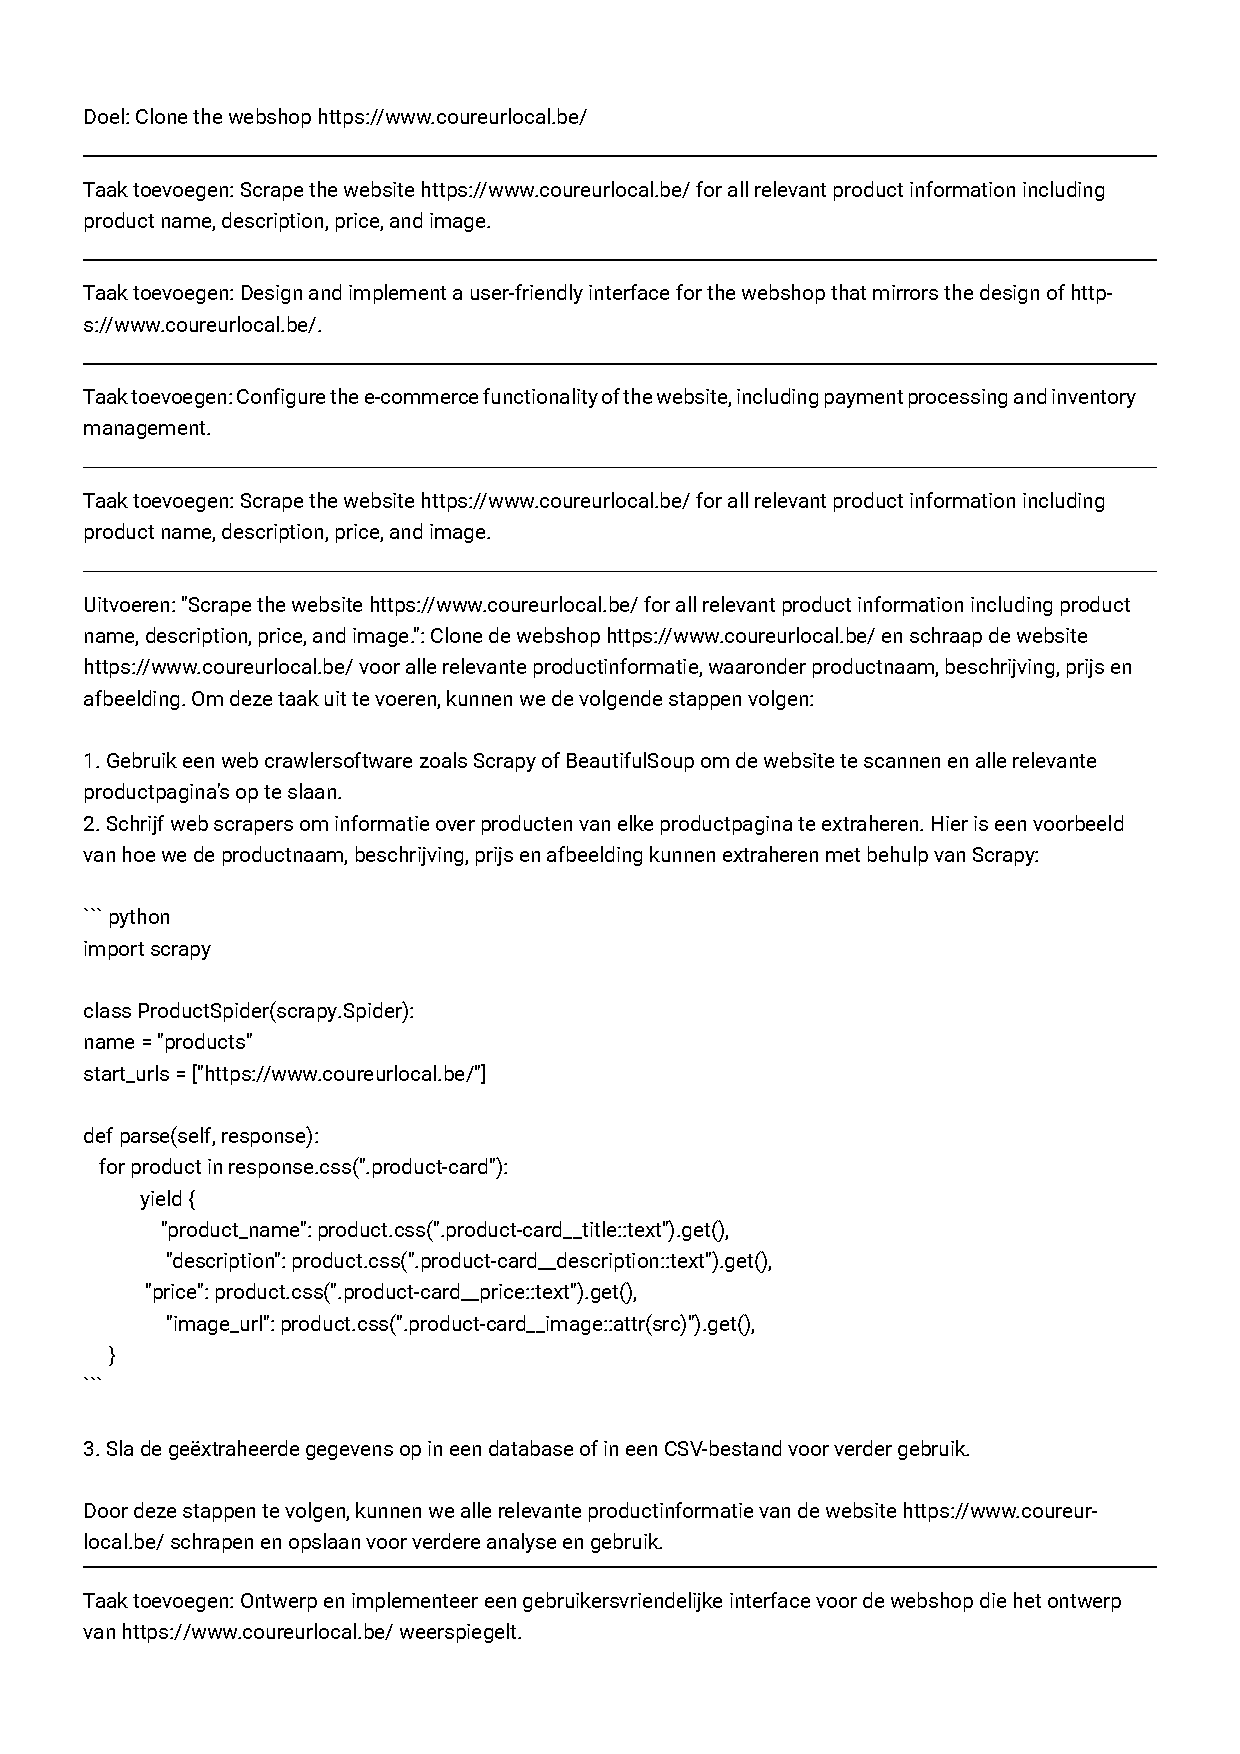
\includepdf[pages=-]{agentGPT_coureur_local.pdf}
%\input{agentGPT_coureur_local.pdf}
%\input{./agentGPT_coureur_local.pdf}:

%%---------- Backmatter, referentielijst ---------------------------------------

\backmatter{}

\setlength\bibitemsep{2pt} %% Add Some space between the bibliograpy entries
\printbibliography[heading=bibintoc]

\end{document}
